\section{Collisionless quantum lattice Boltzmann method \label{sec:cqbm}}
In this chapter we will introduce the reader to our quantum implementation of the collisionless lattice Boltzmann method. We will first describe how the equation can be encoded in the quantum register, and subsequently we will provide the quantum primitive for the streaming, specular reflection and bounce back step. 

\subsection{Quantum register set-up}\label{sec:quantum register set-up}
In order to implement our CQBM approach we first need to define an encoding to give a physically interpretable meaning to quantum basis states. 
In our implementation we define a mapping, where each parameter is assigned to its own set of qubits, which combined form the total qubit register. 
We use the following encoding:
% \begin{equation}
%     \ket{a_{2d} \dots a_1 l_{dN_d} \dots l_{d1} \dots l_{xN_x} \dots l_{x1} v_{N_v} \dots v_1 }
% \end{equation}
\begin{equation}
    \ket{\underbrace{a_{n_a}\dots a_{1}}_{\mathrm{ancillae}} \overbrace{ g_{n_g} \dots g_{1} }^{\mathrm{position}} \underbrace{ v_{n_v} \dots v_1}_{\mathrm{velocity}}}.
\end{equation}

Here, the qubits $a_{n_a}, \dots, a_1$ form the ancillae, with $n_a = 4d-2$, where $d$ is the number of spatial dimensions we are modeling. The $g_{n_g} \dots g_1$ qubits form the positional qubits, with $n_g = \sum_{i=1}^{d}n_{g_i}$, where $n_{g_i}$ is the number of qubits required to number all grid points in the $i$-th spatial dimension. Finally, the qubits $v_{n_v} \dots v_1$ encode the velocity vector, with $n_v = \sum_{i=1}^{d}n_{v_i} $ where $n_{v_i}$ is the number of qubits required number the velocities of the $i$-th dimension. In summary, the total number of qubits required to realize our collisionless quantum Boltzmann method is
\begin{equation}
    a_n + n_g + n_v = 4d-2 + \sum_{i=1}^d (n_{g_i}+n_{v_i}),
\end{equation}
which means that a moderate number of a few dozens to hundred fault-tolerant qubits suffice to enable the solution of two and three-dimensional problems.
The details of the mapping of the ancillae, positional and velocity vectors will be explained more in depth in the following sections. 


\subsubsection{Efficient mapping of velocity vector}
One of the speed-ups our algorithm provides compared to the state-of-the-art is due to our mapping of the velocity vector. 
In each spatial dimension we are working with a predetermined number of discrete velocities $N_{v_i}$. 
For simplicity we will at first only consider the velocity encoding in the one-dimensional case, and call the amount of discrete velocities $N_{v}$. Note that this approach trivially extends to the multi-dimensional case.
As $N_v$ is the number of discrete velocities required, we need $n_{v} = \lceil\log_2\left(N_v\right)\rceil$ qubits to encode all velocities. \\
For our CQBM we restrict ourselves to the case that the set of speeds $\mathcal{U}$ consists of positive and negative values, and for each $u\in \mathcal{U}$ both $|u|\in \mathcal{U}$ and $-|u|\in \mathcal{U}$ will hold. We now define $\mathcal{U}_o = [-u_{\max}, \dots , u_{\max} ]$, the ordered list of speeds from most negative to most positive. 
Let $u_{\min} = \min_k \; |u_k| $ as before and let $\Delta u $ be the distance between the neighboring speeds in $\mathcal{U}_o$, for simplicity we will assume $\Delta u$ is constant between all indices so $\Delta u=\frac{2u_{\max}}{N_v}$. However, we are not restricted to this simplification.  \\
% In the state-of-the-art quantum finite velocity methods (@MATTHIAS, welke term kan ik hier het beste gebruiken) \cite{Todorova2020}, the discrete velocities are mapped to the quantum states as follows: 
% \begin{equation}\label{eq:old_v_encoding}
% \ket{v_{old}} = 
%     \begin{bmatrix}
%     -c_{max} \\
%     -c_{max} +\Delta c  \\
%     \vdots \\
%     -c_{min} \\
%     c_{min}\\
%     c_{min} +\Delta c  \\
%     \vdots \\
%     c_{max}\\
%     \end{bmatrix}.
% \end{equation}
% In such algorithms the velocities are required to control streaming operations and the direction of the velocity needs to be reversed when a particle hits a wall (i.e. $v_i$ becomes $-v_i$). As these are the two requirements, a more efficient encoding of the velocity mapping is possible which saves $\mathcal{O}(n_v)$ multi-controlled not operations in the reflection step. 
% This is due to the fact that in the current implementation, in order to reverse a velocity (i.e. going from the basis state encoding $v_i$ in \eqref{eq:old_v_encoding} to the basis state encoding $-v_i$), each qubit needs to be flipped \cite{Todorova2020}. 
% In practical algorithms such a reversal of velocity needs to be done in a multi-controlled fashion, making each qubit flip rather expensive. \\

We propose the following mapping of the discrete velocities to the quantum state:
\begin{align}
\ket{v_{n_v} \dots v_1} = 
    \begin{bmatrix}
    -u_{\min} \phantom{\, -\Delta u}\\
    -u_{\min} -\Delta u\\
    \vdots \\
    -u_{\max} \phantom{\, -\Delta u}\\
    \phantom{-}u_{\min} \phantom{\, -\Delta u}\\
    \phantom{\,-}u_{\min} +\Delta u  \\
    \vdots \\
    \phantom{-}u_{\max} \phantom{\, +\Delta u}\\
    \end{bmatrix}.\label{eq:our_v}
\end{align}
The motivation of this velocity mapping is that we can flip the direction of the velocity by flipping only one qubit. This can be seen by noting that the distance between the index of velocity $-|u_k|$ and $|u_k|$ in $\mathcal{U}_o$ is precisely $\frac{N_v}{2} = 2^{n_v-1}$, and so we can flip between these two velocities by flipping the most significant qubit which encodes the sign of the velocity vector.% as that represents exactly the $\frac{N_v}{2} = 2^{n_v-1}$ value in binary.\\

This means that we can write the quantum register encoding the velocity in the one dimensional case as: 
\begin{equation}
   \ket{v_{\text{dir}} v_{n_v -1} \dots v_1}.
\end{equation}
In the above expression the first qubit encodes the direction of the velocity (positive or negative in the given dimension), and the next $n_v-1$ qubits encode the magnitude of the velocity. We define $\ket{00 \dots 0}$ to encode $-u_{\min}$, $\ket{00 \dots 1}$ to encode $-u_{\min} - \Delta u$ and $\ket{11 \dots 1}$ to represent $u_{\max}$ etc. It can easily be seen that this leads to a velocity encoding as given in Equation \eqref{eq:our_v}.

\paragraph{Example}\
\normalem
\emph{We give an example of our velocity encoding to show that flipping the direction can be established by flipping only the most significant qubit. Let us consider the 1-dimensional case and say we have $N_v = 8$. Now let $u_1 = u_{\min}$, $u_2 = u_{\min} + \Delta u$ and $u_3 = u_{\min} + 2\Delta u$ etc., then our velocity encoding gives $$\ket{v} = \begin{bmatrix}
-u_1 \\ -u_2\\ -u_3 \\ -u_4\\ \phantom{-}u_1 \\ \phantom{-}u_2\\ \phantom{-}u_3 \\ \phantom{-}u_4 
\end{bmatrix}.$$ Say our particle is traveling with velocity $u_2$, then $\ket{v} = \ket{101}$. Now flipping the most significant qubit gives $\ket{v} = \ket{001}$ which maps to $-u_2$ as required. }\\
% \emph{We will now give an example of our velocity encoding method to show that flipping the velocity direction can be established by flipping only the most significant qubit. Let us consider the 1-dimensional case and say we have $N_v = 8$, then we can encode $\ket{v} = \begin{bmatrix}
% -u_\text{min} \\ -u_\text{min} - \Delta u \\ -u_\text{min} -2\Delta u \\ -u_\text{max} \\ u_\text{min}  + \Delta u \\ u_\text{min} + 2\Delta u \\ u_\text{min} + 3\Delta u \\ u_\text{max}
% \end{bmatrix}$ . Now say our particle is traveling with velocity $u_2$, then $\ket{v} = \ket{101}$, now flipping the most significant bit gives $\ket{v} = \ket{001}$ which maps to $-u_2$. }\\

\ULforem
Extending the above approach to the multidimensional case, the quantum register for the $d$-dimensional velocity becomes: 
\begin{equation}
\ket{v_{\text{dir},d} \dots v_{\text{dir},1} v^d_{n_{v_d}} \dots v^d_{1} v^{d-1}_{n_{v_{d-1}}} \dots v^{d-1}_{1} \dots v^1_{n_{v_1}} \dots v^1_{1}} . 
\end{equation}

Former encodings of the velocity vector for quantum Boltzmann methods were set-up such that in order to flip the velocity of a particle, all qubits encoding the velocity needed to be flipped \cite{Todorova2020}. Our new encoding saves $\mathcal{O}\left ( n \right )$ qubit flips per reflection. Notice that since reflections are usually implemented in multi-control fashion, as described in Section \ref{sec:complete quantum specular reflection step}, this ends up in saving $\mathcal{O}\left (n \right )$ computationally costly operations per reflection. In the appendix we give an in depth complexity analysis and comparison of the different methods.

\subsubsection{Mapping of grid point locations onto qubit states}
The mapping of the grid point locations onto qubit states is rather straightforward. As before, let $\ket{g_{n_g} \dots g_1}$ represent the state of the qubits encoding the grid point location of the particles. Then, we can write the qubits encoding the location more detailed as
\begin{equation}
\ket{g^d_{n_{g_d}} \dots g^d_{1} g^{d-1}_{n_{g_{d-1}}} \dots g^{d-1}_{1} \dots  g^1_{n_{g_1}} \dots g^1_{1}},
\end{equation}
where $g^i_{n_{g_i}} \dots g^i_{1} $ encodes the $i$-th dimension of the location of grid points by representing the binary value of the location. The set-up of the grid is rather straightforward with different grid-points in each dimension and the particles being able to move one step forward and backward in each time step and in each dimension. 


\subsubsection{Ancillae}
The ancillae are the last of the register expressed in Equation \eqref{eq:our_v} and are used within the computation only. 
Each dimension requires one ancilla to keep track of which velocities will be streamed and one ancilla to keep track of the resetting
during the reflection step, furthermore we require $2(d-1)$ ancillae to implement a quantum comparator method that will be used in the reflection step, leading to a total of $4d-2$ ancillae required throughout the computation.
The exact set-up and utilization of the ancillae will be described in Sections \ref{sec:efficient quantum convection operation} and \ref{sec:complete quantum specular reflection step}. 


\subsection{Efficient quantum streaming operation}\label{sec:efficient quantum convection operation}
As described in Section \ref{sec:collisionless boltzmann equation2} the main ingredients of the collisionless quantum Boltzmann method are the streaming and the reflection operations. In this section we will introduce a novel streaming operation based on the Quantum Draper Adder \cite{Draper1998}, which we specialize to an efficient quantum incrementation (decrementation) procedure that is cheaper than those used before \cite{Douglas2009,Fillion-Gourdea2017, Fillion-Gourdea2018,Todorova2020}. \\

\subsubsection{Efficient quantum incrementation (decrementation)}\label{ssec:efficient quantum incr}
An increment (decrement) operation takes a quantum state $\ket{j}$ to the state $\ket{j+1}$ $\left (\ket{j-1} \right )$. This operation is cyclic, meaning that $\ket{2^n-1}$ ($\ket{0}$) gets incremented (decremented) to $\ket{0}$ $\left (\ket{2^n-1} \right )$.  
Let $U_\text{inc}$ ($U_\text{dec}$) express the unitary that increases (decreases) the $n$ qubit state $\ket{j}$: 
\begin{equation}
    U_\text{inc} \ket{j} = \ket{j+1},
\end{equation}
\begin{equation}
    U_\text{dec} \ket{j} = \ket{j-1}.
\end{equation}
This quantum primitive is used in many different quantum algorithm and fields such as Quantum Random Walks and Quantum Computational Fluid Dynamics, to name just a few. In the literature this primitive is typically implemented by cascading multi-controlled NOT operations \cite{Douglas2009,Fillion-Gourdea2017, Fillion-Gourdea2018,Todorova2020, Budinski2021}. While this implementation looks elegant on paper, decomposing multi-controlled NOT operations into gates that are native to quantum computers, i.e., single-controlled NOT gates, will lead to a significant increase of the circuit depth. 

In this section we provide an alternative method leading to a quantum streaming operation which can be implemented more efficiently on real-world quantum computers. The method is inspired by the Quantum Draper Adder (QDA) \cite{Draper1998} and uses the same principle, but in contrast to the regular Drapper adder that computes $\ket{a + b}$, where $a$ and $b$ are natural numbers encoded in a quantum register, in our implementation the phase shift operations are not controlled as the addition by $b=1$ is always known beforehand. As we moreover want our operation to be cyclic, no qubit for holding a potential carry over value is required. We are, to the best of our knowledge, the first to use such a QDA inspired approach for the quantum incrementer (decrementer) and the Appendix we show that it leads to a significant reduction in the amount of CNOT gates required to run the algorithm. \\

Our method can be expressed by the circuit given in Figure \ref{fig:streaming_no_anc}. 
Let $\ket{j}$ be the basis state that we wish to increment (decrement). We claim
\begin{equation} \label{eq:our_adder}
    \ket{j+1} = (QFT)^\dagger U_{P,+} (QFT) \ket{j},
\end{equation} and define 
\begin{equation} \label{eq:def our_adder}
    U_\text{inc}= (QFT)^\dagger U_{P,+} (QFT),
\end{equation} where QFT stands for Quantum Fourier Transform and $U_{P,+}$ will be defined below.
We will now show that \eqref{eq:our_adder} indeed holds. First: 
\begin{equation}
    QFT \ket{j} = \frac{1}{\sqrt{N}}\sum_{k=0}^{N-1} \omega_N^{kj}\ket{k} = \frac{1}{\sqrt{N}} \sum_{k=0}^{N-1} e^{\frac{2 i \pi k j}{N}}\ket{k}.
\end{equation}
Then the circuit $U_{P,+}$ consists of one phase shift gate\footnote{The single qubit phase shift gate can be expressed in matrix form as $P\left ( \theta \right ) = \begin{bmatrix}1 & 0 \\ 0 & e^{i\theta} \end{bmatrix}$.  } per qubit with an angle determined by the qubit number of the qubit to which it is applied. We apply the phase shift gate $P(\theta)$ to the $j$-th qubit\footnote{In this section, for simplicity, we index the qubits ranging from 0 to $n-1$.} with angle
\begin{equation}\label{eq:theta_i}
    \theta_j=\frac{\pi}{2^{n-1-j}} =\frac{\pi 2^{j+1}}{N}.
\end{equation}

So $P(\theta_j)$ gets applied to qubit $j$ and adds amplitude $e^{\frac{i2\pi 2^j}{N}}$ to each basis state for which qubit $j$ is in the state $1$. This means that if we apply the operation $P(\theta_j)$ to each qubit for the basis state $\ket{k}$ it gets multiplied by a factor $e^{\frac{2\pi i k}{N}}$. 

And so we get: 
\begin{equation}
    U_{P,+} (QFT) \ket{j} = \frac{1}{\sqrt{N}} \sum_{k=0}^{N-1} e^{\frac{2 i \pi k j}{N}}e^{\frac{2\pi i k}{N}} \ket{k} = \frac{1}{\sqrt{N}} \sum_{k=0}^{N-1} e^{\frac{2 i \pi k (j+1)}{N}}\ket{k} .
\end{equation}

It then directly follows that: 
\begin{equation}
    (QFT)^\dagger U_{P,+} (QFT) \ket{j} = QFT^\dagger \frac{1}{\sqrt{N}} \sum_{k=0}^{N-1} e^{\frac{2 i \pi k (j+1)}{N}}\ket{k}  = \ket{j+1}.
\end{equation}
In other words our proposed algorithm increases each basis state by $1$, whereby the periodic property of $e^{i\theta}$ ensures that the so-defined increase operation is cyclic. Naturally the decrease operation becomes:
\begin{equation}
    \ket{j} =  \left ( (QFT)^\dagger U_{P,+} (QFT) \right )^\dagger \ket{j+1} = (QFT)^\dagger U_{P,+}^\dagger (QFT) \ket{j+1}.
\end{equation}
Since $U_{P,+}$ consists of a layer of phase shift gates taking the conjugate transpose is equal to shifting the angles to their negative counterparts. So for $U_{P,+}^\dagger$ we apply the phase shift gate $P(-\theta_j)$ to the $j$-th qubit with angle $-\theta_j$, where $\theta_j$ is as given in \eqref{eq:theta_i}.
For simplicity we define $U_{P,-} = U_{P,+}^\dagger$. It then follows that: 
\begin{equation}
    U_{\text{dec}} = (QFT)^\dagger U_{P,-} (QFT).
\end{equation}
 



% \subsection{Proposed incrementation (decrementation) method}
% Our incrementation method can be expressed by the circuit as given in figure \ref{}. 
% Let $\ket{j}$ be the basis state to which we apply the qubit, the we claim: 
% \begin{equation} \label{eq:our_adder}
%     \ket{j+1} = QFT^\dagger U_P QFT \ket{j}.
% \end{equation}

% We will now show that \eqref{eq:our_adder} holds. First: 
% \begin{equation}
%     QFT \ket{j} = \frac{1}{\sqrt{N}}\sum_{k=0}^{N-1} \omega_N^{kj}\ket{k} = \frac{1}{\sqrt{N}} \sum_{k=0}^{N-1} e^{\frac{2 i \pi k j}{N}}\ket{k}.
% \end{equation}
% Then the circuit $U_P$ consists of one phase shift gate per qubit with an angle determined by which qubit it is applied to. We apply the phase shift gate $P(\theta)$ to the $i$-th qubit with angle
% \begin{equation}
%     \theta_i=\frac{\pi}{2^{n-1-i}} =\frac{2\pi 2^i}{N}.
% \end{equation}

% So $P(\theta_i)$ gets applied to qubit $i$ and adds amplitude $e^{\frac{2\pi 2^i}{N}}$ to each basis state for which qubit $i$ is in the state $1$. This means that if we apply this operation $P(\theta_i)$ to each basis state $\ket{k}$ it gets multiplied by a factor $e^{\frac{2\pi i k}{N}}$. 

% And so we get: 
% \begin{equation}
%     U_P QFT \ket{j} = \frac{1}{\sqrt{N}} \sum_{k=0}^{N-1} e^{\frac{2 i \pi k j}{N}}e^{\frac{2\pi i k}{N}} \ket{k} = \frac{1}{\sqrt{N}} \sum_{k=0}^{N-1} e^{\frac{2 i \pi k (j+1)}{N}}\ket{k} .
% \end{equation}

% It then directly follows that: 
% \begin{equation}
%     QFT^\dagger U_P QFT \ket{j} = QFT^\dagger \frac{1}{\sqrt{N}} \sum_{k=0}^{N-1} e^{\frac{2 i \pi k (j+1)}{N}}\ket{k}  = \ket{j+1}.
% \end{equation}
% And so our proposed algorithm increases each basis state by $1$. Note that from the periodic properties of $e^{i\theta}$ that this increase operation is cyclic. Naturally the decreasing operation becomes:
% \begin{equation}
%     \ket{j} =  (QFT)^{-1} U_P^{-1} (QFT^\dagger)^{-1} \ket{j+1} = (QFT^\dagger) U_P^\dagger (QFT) \ket{j+1}.
% \end{equation}
% Since $U_P$ consists of a layer of phase shift gates taking the complex conjugate is equal to shifting the angles to their negative counter parts. So for $U_P^\dagger$ we apply the phase shift gate $P(-\theta)$ to the $i$-th qubit with angle
% \begin{equation}
%     \theta_i=\frac{\pi}{2^{n-1-i}} =\frac{2\pi 2^i}{N}.
% \end{equation}




\subsubsection{Streaming step}\label{ssec:convection step}
In the streaming step particles migrate from one discrete point in space to another. 
In each time step the particles that travel at a discrete speed such that they reach the next grid point in the current time step get incremented (or decremented) one position in space. The list of speeds for which particles traveling at that specific speed need to be incremented (decremented) at a particular time step is pregenerated by the CFL counter as described in Section \ref{ssec:cfl_counter}. Then, controlled on their speeds, the particles are incremented (decremented) one position at a time. This means that we implement the quantum incrementation (decrementation) method as described in the last section in a controlled fashion as will be detailed below.  \\

First of all we notice that we do not have to control the entire incrementation (decrementation) primitive from Section \ref{ssec:efficient quantum incr}. Since the incrementation (decrementation) step consists of the QFT followed by a layer of phase shift gates followed by QFT$^\dagger$, it suffices to only control the layer of phase shift gates on the speed of the particles, as the QFT and QFT$^\dagger$ operations naturally cancel out each other. Furthermore, since the incrementation and decrementation step are performed directly after each other on the same qubits, we do not have to perform a QFT$^\dagger$ operation after the phase shift gates of the incrementation step, as this would cancel out with the QFT operation at the start of the decrementation step.  \\

Second, we notice that if we make use of an ancilla we can perform the incrementation and decrementation operations for all speeds that take a step in the current time step using a single operation in a given dimension $i$. 

To this end, let $|u_k|$ be (one of) the absolute values of the speeds for which the streaming step is to be performed at a certain point in the algorithm. Then in each dimension $i$ we need to increment the particles traveling at speed $u^{(i)} = \pm |u_k|$. Because of the way the binary encodings of $u_k$ and $-u_k$ are related in each dimension, we first perform a controlled-NOT operation between the $n_{v_i}-1$ qubits determining the absolute value of the velocity and an ancilla qubit $a_{u,i}$. If there are multiple values $k$ such that particles traveling at speed $\pm u_k$ need to be incremented in the given time step, this process is applied to all such $k$. This means that we simply flip the value of the ancilla qubit $a_{u,i}$ to 1 for all the registers of the particles traveling at a speed such that they should reach the next grid point in dimension $i$ in the current time step. We then use the ancilla $a_{u,i}$ in combination with the directional velocity qubit $v_{\text{dir},i}$ to increase or decrease the position of the correct particles in space in each dimension $i$. 
In practice, the streaming step using the ancilla qubits $a_{u,i}$ should be implemented as it leads to a more efficient algorithm, due to the fact that we now perform the incrementation (decrementation) primitive for all the particles taking a step in the given time step using a single operation. 

\begin{figure}
    \centering
    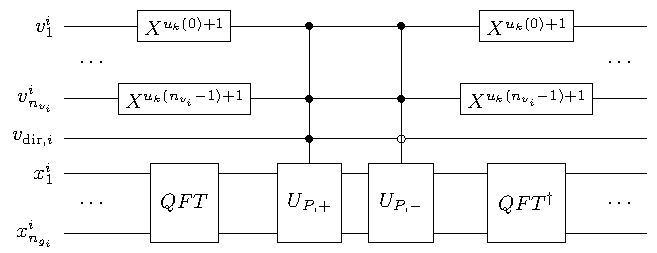
\includegraphics{imgs/cqlbm/streaming no anc_2.pdf}
%     \[\Qcircuit @C=1.3em @R=1em {
% %& & & & & \mbox{Rigetti generated amplitude amplification circuit} & & & & & \\
% &\lstick{v^i_1} & \qw & \gate{X^{u_{k}(0)+1}} & \qw & \ctrl{4} & \ctrl{4} & \qw & \gate{X^{u_{k}(0)+1}} & \qw & \qw\\
% &\lstick{} & \cdots & & & & & & & \cdots & \\
% &\lstick{v^i_{n_{v_i}}} & \qw & \gate{X^{u_{k}(n_{v_i}-1)+1}} & \qw & \ctrl{2} & \ctrl{2} & \qw & \gate{X^{u_{k}(n_{v_i}-1)+1}} &\qw &\qw\\
% &\lstick{v_{\text{dir},i}} & \qw & \qw & \qw & \ctrl{1} &\ctrlo{1} & \qw & \qw & \qw & \qw\\
% &\lstick{x^i_1} & \qw & \qw & \multigate{2}{QFT} & \multigate{2}{U_{P,+}} &\multigate{2}{U_{P,-}}  & \multigate{2}{QFT^\dagger} & \qw & \qw & \qw\\
% &\lstick{} & \cdots & &  &  & & & & \cdots &  \\
% &\lstick{x^i_{n_{g_i}}} & \qw & \qw & \ghost{QFT} & \ghost{U_{P,+}} &\ghost{U_{P,-}} & \ghost{QFT^\dagger} & \qw & \qw & \qw\\}\]
    \caption{Circuit representation of the proposed streaming step in dimension $i$ for one speed $|u_k|$ without extra ancilla qubits.}
    \label{fig:streaming_no_anc}
\end{figure}


\begin{figure}
    \centering
    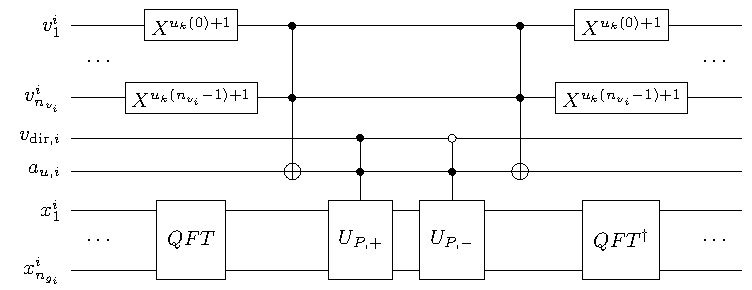
\includegraphics{imgs/cqlbm/streaming ancilla.pdf}
% \[
% \Qcircuit @C=1.3em @R=1em {
% %& & & & & \mbox{Rigetti generated amplitude amplification circuit} & & & & & \\
% \lstick{v^i_1} & \qw & \gate{X^{u_{k}(0)+1}} & \ctrl{4}  &\qw & \qw & \ctrl{4} & \gate{X^{u_{k}(0)+1}} & \qw & \qw\\
% \lstick{} & \cdots & & & & & & & \cdots & \\
% \lstick{v^i_{n_{v_i}}} & \qw & \gate{X^{u_{k}(n_{v_i}-1)+1}} & \ctrl{2}   &\qw  & \qw & \ctrl{2} & \gate{X^{u_{k}(n_{v_i}-1)+1}} &\qw &\qw\\
% \lstick{v_{\text{dir},i}} & \qw & \qw &  \qw & \ctrl{1} & \ctrlo{1} & \qw & \qw & \qw & \qw\\
% \lstick{a_{u,i}} & \qw & \qw & \targ  & \ctrl{1} & \ctrl{1} & \targ & \qw & \qw & \qw \\
% \lstick{x^i_1} & \qw  & \multigate{2}{QFT}  & \qw & \multigate{2}{U_{P,+}} &\multigate{2}{U_{P,-}} &\qw & \multigate{2}{QFT^\dagger} & \qw & \qw\\
% \lstick{} & \cdots &  & &  & & & & \cdots &  \\
% \lstick{x^i_{n_{g_i}}} & \qw & \ghost{QFT}   & \qw & \ghost{U_{P,+}} &\ghost{U_{P,-}} & \qw & \ghost{QFT^\dagger} & \qw & \qw\\
% }\] 
    \caption{Circuit representation of the proposed streaming step in dimension $i$ for one speed $|u_k|$ with ancilla qubit. Note that here we reset the $a_{u,i}$ ancilla after the streaming step. In the proposed algorithm this ancilla will only be reset after the reflection operation has been performed. }
    \label{fig:streaming_anc}
\end{figure}

\begin{figure}
    \centering
    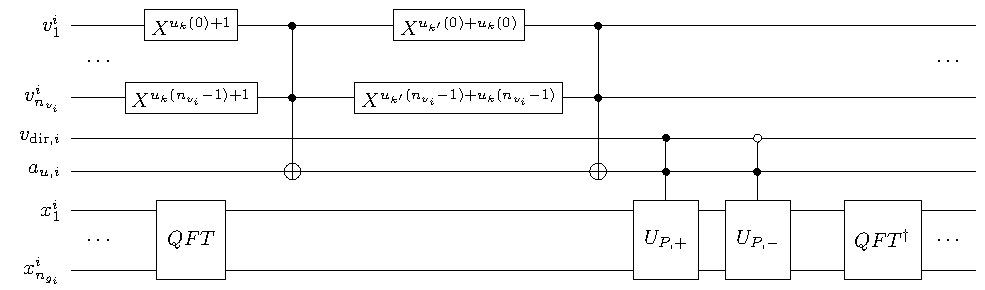
\includegraphics[scale = .75]{imgs/cqlbm/streaming k and k prime.pdf}
% \[
% \Qcircuit @C=1.3em @R=1em {
% %& & & & & \mbox{Rigetti generated amplitude amplification circuit} & & & & & \\
% \lstick{v^i_1} & \qw & \gate{X^{u_{k}(0)+1}} & \ctrl{4} &\qw & \gate{X^{u_{k+1}(0)+u_{k}(0)}} & \ctrl{4}  &\qw & \qw & \qw & \qw& \qw & \qw\\
% \lstick{} & \cdots & & & & & & & & & & \cdots & \\
% \lstick{v^i_{n_{v_i}}} & \qw & \gate{X^{u_{k}(n_{v_i}-1)+1}} & \ctrl{2} & \qw & \gate{X^{u_{k+1}(n_{v_i}-1)+u_{k}(n_{v_i}-1)}} & \ctrl{2}   &\qw  & \qw & \qw & \qw &\qw &\qw\\
% \lstick{v_{\text{dir},i}} & \qw & \qw &  \qw & \qw & \qw &  \qw & \ctrl{1} & \ctrlo{1} & \qw & \qw & \qw & \qw\\
% \lstick{a_{u,i}} & \qw & \qw & \targ & \qw & \qw & \targ  & \ctrl{1} & \ctrl{1} & \qw & \qw & \qw & \qw \\
% \lstick{x^i_1} & \qw  & \multigate{2}{QFT} & \qw & \qw & \qw  & \qw & \multigate{2}{U_{P,+}} &\multigate{2}{U_{P,-}} &\qw & \multigate{2}{QFT^\dagger} & \qw & \qw\\
% \lstick{} & \cdots &  & & &  & &  & & & & \cdots &  \\
% \lstick{x^i_{n_{g_i}}} & \qw & \ghost{QFT} & \qw & \qw & \qw  & \qw & \ghost{U_{P,+}} &\ghost{U_{P,-}} & \qw & \ghost{QFT^\dagger} & \qw & \qw\\
% }\] 
    \caption{Circuit representation of the proposed streaming step in dimension $i$ for two speeds $|u_k|$ and $|u_{k^\prime}|$ with ancilla qubit. Note how the proposed ancilla qubit allows to perform the streaming $U_{P,+}$ for both speeds in one operation. Here we do not reset the ancilla qubit $a_{u,i}$ after the streaming step, as in the proposed algorithm this ancilla will only be reset after the reflection operation has been performed.}
    \label{fig:streaming_anc two}
\end{figure}

% \begin{figure}
%     \centering
% \[
% \Qcircuit @C=1.3em @R=1em {
% %& & & & & \mbox{Rigetti generated amplitude amplification circuit} & & & & & \\
% \lstick{v_0} & \qw & \gate{X^{u^j_0+1}} & \ctrl{4} &\qw & \gate{X^{u^{j+1}_0+1}} & \ctrl{4}  &\qw & \qw & \ctrl{4} & \gate{X^{u^j_0+1}} & \qw & \qw\\
% \lstick{} & \cdots & & && & & & & & & \cdots & \\
% \lstick{v_m} & \qw & \gate{X^{u^j_m+1}} & \ctrl{2} & \qw & \gate{X^{u^{j+1}_m+1}} & \ctrl{2}   &\qw  & \qw & \ctrl{2} & \gate{X^{u^j_m+1}} &\qw &\qw\\
% \lstick{v_\text{dir}} & \qw & \qw &  \qw & \qw & \qw &  \qw & \ctrl{1} & \ctrlo{1} & \qw & \qw & \qw & \qw\\
% \lstick{a_{u,i}} & \qw & \qw & \targ & \qw & \qw & \targ  & \ctrl{1} & \ctrl{1} & \targ & \qw & \qw & \qw \\
% \lstick{x_0} & \qw  & \multigate{2}{QFT} & \qw & \qw & \qw  & \qw & \multigate{2}{U_{P,+}} &\multigate{2}{U_{P,-}} &\qw & \multigate{2}{QFT^\dagger} & \qw & \qw\\
% \stick{} & \cdots &  & & &  & &  & & & & \cdots &  \\
% \lstick{x_m} & \qw & \ghost{QFT} & \qw & \qw & \qw  & \qw & \ghost{U_{P,+}} &\ghost{U_{P,-}} & \qw & \ghost{QFT^\dagger} & \qw & \qw\\
% }\] 
%     \caption{Circuit representation of the proposed streaming step for one speed $|u_j|$ with ancilla qubit. If there are multiple speeds $|u_j|$ for which the particles traveling at that speed reach the next grid point in the timestep, we simply also flip the ancilla qubit $a_{u,i}$ for those speeds before performing the controlled $U_{P,+}$ and $U_{P,-}$ operations.}
%     \label{fig:streaming_anc}
% \end{figure}


Let ${u_{k}(n)}$ represent the value of the $n$-th bit when representing the index of the speed $u_{k}$ in the velocity vector\footnote{For example, assume we want to control on the speed being equal to $u_2$, let $\ket{u_2} = \ket{v_\text{dir}v_m \dots v_0} = \ket{10010}$. Then ${u_{2}(0)} = 0$ and ${u_{2}(1)} = 1$ etc. }. Then, we perform the operation $X^{u_k(l-1)+1}$ on each qubit $v^i_l \in \{v^i_{1}, \dots, v^i_{n_{v_i}}\}$ followed by the multi-controlled NOT operation between the $v^i_{1} \dots v^i_{n_{v_i}}$ qubits and the $a_{u,i}$ qubit for all speeds $|u_k|$ that take a step in the given time step, before performing the controlled streaming operations. Notice that we need to make sure to apply the $X^{u_k(l-1)+1}$ operations again after performing the multi-controlled NOT, to reset the speeds to their original states before we apply the $X^{u_{k^\prime}(l-1)+1}$ associated with the next speed $u_{k^\prime}$ for which the particles need to be streamed in this timestep. Furthermore, notice that we can simply combine these subsequent operations and get $X^{u_k(l-1)+1+u_{k^\prime}(l-1)+1} = X^{u_k(l-1)+u_{k^\prime}(l-1)}$ to be applied before the multi-controlled NOT operation to set the ancilla $a_{u,i}$ for the speed $u_{k^\prime}$. Figure \ref{fig:streaming_no_anc} shows the circuit of the streaming step without the ancilla $a_{u,i}$. Figure \ref{fig:streaming_anc} shows what the circuit of the streaming step with the ancilla $a_{u,i}$ looks like when streaming the particles with speed $u_k$ in dimension $i$. Figure \ref{fig:streaming_anc two} shows how using the ancilla qubit $a_{u,i}$ enables streaming the particles with several (in this example two) speeds $u_k$ and $u_{k^\prime}$ in dimension $i$ using a single $U_{p,+}$ and $U_{p,-}$ operation. In Figure \ref{fig:streaming_anc two} we do not reset the ancilla qubit $a_{u,i}$ after performing the streaming step, as in practice these will only get reset after the specular reflection step of the algorithm has been performed. 

In the above we have presented the streaming algorithm for a single dimension $i$. When working with multiple dimensions we perform the exact same operations in each dimension. Note how the streaming of the particle in the different dimensions can be applied to the qubits simultaneously, as different qubits are involved in the streaming step for each dimension. 
% Furthermore, we will make use of the state of these ancilla qubits $a_{u,i}$ in the specular reflection step of the algorithm, exploiting that now we can use these states in this step ``for free''. This means that in practice we do not reset the ancilla qubits $a_{u,i}$ after the specular reflection step, but we wait with doing this until after the specular reflection step has been completed. In Figure \ref{fig:streaming_anc two} we present how the streaming method with ancilla qubit can be used to stream particles of several (in this case two) speeds $u_j, u_{j+1}$ at the same time. In this Figure we also show what the streaming step implemented in the algorithm will look like, since we do not reset the ancilla qubit $a_{u,i}$ as in practice those will only be reset after the reflection step has been performed.
% % See Figure \ref{} for the exact quantum building block that is applied to the qubits in the quantum algorithm in the streaming step.\\
% In Figures \ref{fig:streaming_no_anc} and \ref{fig:streaming_anc} we give a circuit representation of our proposed streaming algorithm (including cancellation of interior QFT$^\dagger$ QFT pairs) both with and without the extra ancilla qubit when streaming the particles of only one speed $u_j$. In Figure \ref{fig:streaming_anc two} we present how the streaming method with ancilla qubit can be used when particles of multiple (in this case two) speeds $u_j, u_{j+1}$ are streamed at the same time. In this Figure we also show what the streaming step implemented in the algorithm will look like, since we do not reset the ancilla qubit $a_{u,i}$ as in practice those will only be reset after the reflection step has been performed.
% % @MEREL make this picture, misschien ook in the quantum overview total blahblah hoofdstuk?


% \subsection{CFL counter}\label{ssec:cfl_counter implemented}

% Now that we have described quantum circuits that implement a streaming step for particles of a specific velocity in each time step, we must also explain how to use these quantum circuits as blocks to build up the total algorithm. 

% In each time step $m$ of the algorithm we need to make sure that the particles with the right velocities are incremented (decremented) one step in space. We do this by letting the streaming step of the algorithm be built up of quantum circuits as described in Section \ref{ssec:convection step} for the speeds $u \in \mathcal{U}$ reaching the next grid point. In order for quantum algorithm to be efficiently implementable for variable velocity vectors, we need to describe an algorithm to build up our total algorithm using these quantum blocks. 

% We do this by making use of the CFL counter as described in Section \ref{ssec:cfl_counter}. Specifically, we first calculate the values $\Delta t_m$ as described in Equation \eqref{eq:delta_t} on a classical computer before creating the quantum circuit. When calculating the values $\Delta t_m$, we simultaneously keep track of which velocities reach the next grid point in each time step. This list is finally used to build up the correct quantum circuit, where in each time step the right particles get streamed to the next grid point. 

% To do this we use the following algorithm:  
% \begin{minted}{python}
% def time_series(Nv, M):
%     steps = 0
%     C = np.zeros(int(Nv/2))
%     v_p = np.arange(.5, Nv/2+ .5, 1)
%     recip = np.reciprocal(v_p)
%     ones = np.ones(int(Nv/2))
%     speed_ctrl = []
%     for i in range(M):
%         mult = np.multiply(ones - C,recip)
%         argmin = np.argmin(mult)
%         mini = mult[argmin]
%         C = C + mini*v_p
%         vels = []
%         for i in range(Nv/2): 
%             if round(C[i],6)== 1:
%                 C[i]=0
%                 vels.append(i)
%         C[argmin] = 0
%         speed_ctrl.append(vels)
%         steps+=1
%         if np.count_nonzero(np.round(C,6)==0.) + np.count_nonzero(np.round(C,6) == 1.) == int(Nv/2):
%             break
%     return speed_ctrl
% \end{minted}

% Clearly in this implementation we need $M N_v$ steps to create the time series, where $M$ is a pre-determined hyperparameter. So the complexity of this calculation is linear. In \cite{Todorova2020} they show that the value of $M$ is observed to grow linearly in $N_v$ with a factor 4, leading to the approximation 
% \begin{equation}
%     M \approx 4 N_v,
% \end{equation}
% so the complexity of calculating the right incrementation step is estimated to be quadratic in $N_v$. And in practice can be done quickly and efficiently on a classical computer. 



% \subsubsection{Multi-dimensional case}
% The general extension to the multi-dimensional case is trivial. Note that since we encode the velocities of the different dimensions in the same qubits, using extra qubits to keep track of the dimensions, we can exploit this in the case that the velocities are the same in each dimension.


% \[
% \Qcircuit @C=1.3em @R=1em {
% %& & & & & \mbox{Rigetti generated amplitude amplification circuit} & & & & & \\
% \lstick{v_0} & \qw & \gate{X^{v^i_0}} & \ctrl{5} &\qw & \qw & \ctrl{5} & \gate{X^{v^i_0}} & \qw & \qw\\
% \lstick{} & \cdots & & & & & & & \cdots & \\
% \lstick{v_m} & \qw & \gate{X^{v^i_m}} & \ctrl{3} &\qw & \qw & \ctrl{3} & \gate{X^{v^i_0}} &\qw &\qw\\
% \lstick{v_{dir}} & \qw & \qw & \qw & \ctrl{2} & \ctrlo{2} & \qw & \qw & \qw & \qw\\
% \lstick{v_{dim}} & \qw & \qw & \qw & \qw & \qw & \qw & \qw & \qw & \qw\\
% \lstick{a_{u,i}} & \qw & \qw & \targ & \ctrl{1} & \ctrl{1} & \targ & \qw & \qw & \qw \\
% \lstick{x_0} & \qw & \qw & \qw & \multigate{2}{incr} &\multigate{2}{decr} &\qw & \qw & \qw & \qw\\
% \stick{} & \cdots & & &  & & & & \cdots &  \\
% \lstick{x_m} & \qw & \qw & \qw & \ghost{incr} &\ghost{decr} & \qw & \qw & \qw & \qw\\
% \lstick{y_0} & \qw & \qw & \qw & \multigate{2}{incr} &\multigate{2}{decr} &\qw & \qw & \qw & \qw\\
% \stick{} & \cdots & & &  & & & & \cdots &  \\
% \lstick{y_m} & \qw & \qw & \qw & \ghost{incr} &\ghost{decr} & \qw & \qw & \qw & \qw\\
% }\] 





\subsection{Quantum specular reflection step}\label{sec:complete quantum specular reflection step}
After the completion of the streaming operation particles that come into contact with an obstacle and have virtually moved into it have to change their travel path; See Section \ref{ssec:class_reflection}. 

\normalem
Here, we propose a novel and fail-safe approach to the quantum reflection operation. 
First, the particles that virtually traveled into the obstacle have their velocity direction reversed in the direction normal to the wall encountered. 
Afterwards, these particles are placed back into the flow domain. As a result of both operations, the particle is located in the correct grid point and travels in the right physical direction in the next time step.
% In order to achieve this we need to carefully analyze the different cases possible for particle-wall interaction and find a unitary method that portrays the correct behavior in all separate cases. 

To achieve this there are some corner cases that need to be taken into account explicitly to avoid incorrect reflections, furthermore we make sure that there are no particles residing inside the object at the end of a time step. 
% For readability we will define our method for the 2-dimensional case below and give the n-dimensional abstraction in the appendix. @MEREL zou wel vet zijn als ik het naar n-dimensies kan vertalen & bewijzen :D \\

% In order to show that our method leads to the correct result for all possible particle wall interaction we will consider two separate cases. In the first case we consider the interaction of a particle with a wall, in a grid point inside the wall that is not a corner point. In the second case we will consider the more interesting case, of when a particle hits the wall in a so-called corner point. 


\subsubsection{Specular reflection steps - requirements and possible breakdown cases}
% Section \ref{ssec:class_reflection} provides the overview of what is required to happen in the reflection step. In this section we will go over how these requirements translate into the quantum implementation, and which possible breakdown cases must be taken into account. Strategies to mitigate this erroneous behavior will be presented in Section \ref{ssec:Correct Reflection}.
In this section, we translate the general procedure of the reflection step into a concrete quantum algorithm. Strategies to mitigate the erroneous behavior that might occur for the different corner cases will be discussed on Section \ref{ssec:Correct Reflection}

First we need to identify particles that have reached a grid point inside the obstacle, to ensure that they are placed back into the fluid domain before the start of the next streaming step.
This means that controlled on the current location of the particles (namely inside the obstacle), we set them back onto a grid point outside of the obstacle. Performing such an operation on a quantum computer is, however, far from trivial since we cannot alter the state of certain qubits controlled on their own states, as this would constitute a non-unitary operation. 
In our case this means that we cannot simply alter the position of the particles in space based on their current position, as that would be precisely attempting an operation on some qubits controlled by themselves. 

A way to overcome this is to use a system of ancillae to facilitate this back placement. This, however, introduces a new complexity since the ancillae would also have to be reset after the positional move has been performed in order to be usable in the next time step.
The resetting of the ancillae to their original position is nontrivial because we clearly cannot use the original requirements to simply flip the ancillae back, as the original control states were positional and we used the ancillae to control a positional change. Instead, we will have to reset the ancillae based on the new location of the particles in combination with their direction and velocities, i.e., we reverse engineer the particles' previous position. 

Another nontrivial aspect of the specular reflection step is to implement it such that all of the reflections are physically correct and we do not encounter unphysical behavior around the corner points. 
If one were to simply reflect the velocity in the $y$-direction upon hitting a $y$-wall and the velocity in the $x$-direction upon hitting an $x$-wall, incorrect behavior around the corner points will emerge. This is because corner points are points inside the object that are part of walls in multiple directions, i.e., in the two-dimensional case they are part of both an $x$-wall and a $y$-wall. 
What will happen in a non-fail-safe implementation of the specular reflection step is that particles hitting such a grid point coming through just the $x$- or $y$-wall have their velocities reflected in both directions, instead of only the one orthogonal to the wall they came through. 

Figure \ref{fig:example_wrong} gives an example of what can go wrong in a non-fail-safe implementation of the specular reflection step.
We see that in the cases of the green arrows the behavior is correct, as the velocity is reflected in both the $x$- and $y$-direction since the particle hits both an $x$- and $y$-wall. For the case of the blue arrows we see that the behavior is also correct, since the velocity parallel to the wall is zero in this case, therefore reflecting the velocity in this direction has no effect. However, for any particle approaching the corner point from another direction, such as the red arrow, the reflection based on a non-fail-safe implementation will certainly be wrong.  This is due to the fact that such a particle hits a point associated to both an $x$-wall \emph{and} a $y$-wall, even though physically it can easily be seen that the particle only hits either an $x$- \emph{or} a $y$-wall. In a non-fail-safe reflection operation this means that the velocity of the particle is erroneously reversed in both the $x$- \emph{and} the $y$-direction. When considering the shape of the wall and the direction of the particle, it is clear that in these cases only one of the two velocity components should be flipped, namely the velocity component orthogonal to the wall that the particle hits. 
%This leads to the majority of the particles that hit a corner point getting reflected erroneously in a non-fail-safe implementation. 

% Finally we need to consider the possible erroneous behaviors that might occur when $c_\text{rel} >1$ as described in Section \ref{ssec:case2 refl}. Specifically we need to ensure a particle gets reflected when it hits a wall but never actually reaches a grid point inside the object and we need to ensure a particle gets reflected in the correct dimension when a corner point is hit in such cases. 

% Since we already have to make use of extra ancillae to facilitate moving the particles out of the material before the end of the time step, we can use these same ancillae to keep track of which velocity directions should be reflected when a particle hits the object in the corner points. This avoids the problem shown in Figure \ref{fig:example_wrong}, that occurs in the specular reflection step when we do not explicitly keep track of which velocities should be reflected.  
% This does mean that we can only reset the ancillae $a_{v,i}$ after the specular reflection step, and not directly after performing the streaming operation. \\


\begin{figure}
    \centering
    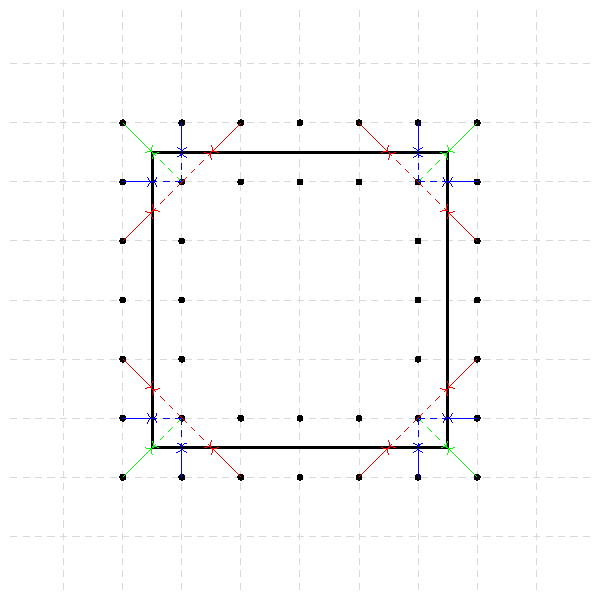
\includegraphics[]{imgs/cqlbm/wrong reflection example.pdf}
    % \begin{tikzpicture}
    % \draw[help lines, color=gray!30, dashed] (-4.9,-4.9) grid (4.9,4.9);
    % \draw[-,color=black] (-2.5,-2.5) -- (-2.5,2.5);
    % \draw[-,color=black] (-2.5,-2.5) -- (2.5,-2.5);
    % \draw[-,color=black] (2.5,-2.5) -- (2.5,2.5);
    % \draw[-,color=black] (-2.5,2.5) -- (2.5,2.5);
    % \foreach \j in {0,...,6}
    % {
    %     \foreach \i in {0,1}
    %     {
    %         \node at (-3+\i,-3+\j)[circle, fill, color = black, inner sep=1pt]{};
    %         \node at (2+\i,-3+\j)[circle, fill, color = black, inner sep=1pt]{};
    %     }
    % }
    % \foreach \j in {0,1}
    % {
    %     \foreach \i in {0,...,4}
    %     {
    %         \node at (-1+\i,-3+\j)[circle, fill, color = black, inner sep=1pt]{};
    %         \node at (-1+\i,2+\j)[circle, fill, color = black, inner sep=1pt]{};
    %     }
    % }


    % \foreach \i in {0,1}
    % {
    %     \draw[->, color=green] (-6*\i+3,-6*\i+3) -- (-5*\i+2.5,-5*\i+2.5);
    %     \draw[->, color=green] (6*\i-3,-6*\i+3) -- (5*\i-2.5,-5*\i+2.5);
        
    %     \draw[->, dashed, color=green] (2-4*\i,2-4*\i) --  (-5*\i+2.5,-5*\i+2.5);
    %     \draw[->, dashed, color=green] (-2+4*\i,2-4*\i) -- (5*\i-2.5,-5*\i+2.5);
        
        
        
    %     \draw[->, dashed, color=blue] (2,2) --  (2.5-.5*\i,2+.5*\i);
    %     \draw[->, color=blue] (3-1*\i,2+\i) -- (2.5-.5*\i,2+.5*\i) ;
    %     %\draw[->, color=blue] (2,2) --  (2+1*\i,3-\i);
        
    %     \draw[->, dashed, color=blue] (-2,2) --  (-2-.5*\i,2.5-.5*\i);
    %     \draw[->, color=blue] (-2-1*\i,3-\i) --  (-2-.5*\i,2.5-.5*\i);
        
    %     \draw[->, dashed, color=blue] (-2,-2) --  (-2-.5*\i,-2.5+.5*\i);
    %     \draw[->, color=blue] (-2-1*\i,-3+\i) --  (-2-.5*\i,-2.5+.5*\i);
        
    %     \draw[->, dashed, color=blue] (2,-2) --  (2+.5*\i,-2.5+.5*\i);
    %     \draw[->, color=blue] (2+\i,-3+\i) -- (2+.5*\i,-2.5+.5*\i);
        
    %     %\draw[->, color=red] (2,2) --  (3-2*\i,1+2*\i);
    %     \draw[->, dashed, color=red] (2,2) --  (2.5 -\i,1.5+\i);
    %     \draw[->,  color=red] (3 -2*\i,1+2*\i) --  (2.5 -\i,1.5+\i);
        
        
    %     \draw[->, dashed, color=red] (-2,2) --  (-2.5+\i,1.5+\i);
    %     \draw[->, color=red] (-3+2*\i,1+2*\i) -- (-2.5+\i,1.5+\i);
        
    %     \draw[->, dashed, color=red] (-2,-2) --  (-2.5+\i,-1.5-\i);
    %     \draw[->, color=red] (-3+2*\i,-1-2*\i) --  (-2.5+\i,-1.5-\i);
        
    %     \draw[->, dashed, color=red] (2,-2) --  (2.5-\i,-1.5-\i);
    %     \draw[->, color=red] (3-2*\i,-1-2*\i) --  (2.5-\i,-1.5-\i);
    % }
    % \end{tikzpicture}
    \caption{Illustration of the different cases of specular reflection at the corner points of an obstacle. While particles traveling into the obstacle along the blue and green velocity trajectories are reflected correctly even by non-fail-safe reflection algorithms, particles approaching the corner points along the red-arrow trajectories require special treatment as is done in our fail-safe specular reflection algorithm.
 }
    
    \label{fig:example_wrong}
\end{figure}



% \begin{figure}[h]
%     \centering
%     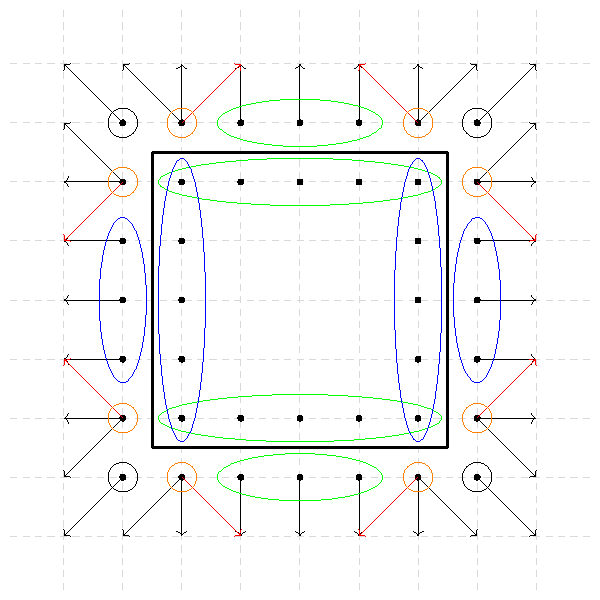
\includegraphics[width=.5\textwidth]{imgs/cqlbm/correct reflections.pdf}
%     % \begin{tikzpicture}
%     % \draw[help lines, color=gray!30, dashed] (-4.9,-4.9) grid (4.9,4.9);
%     % \draw[-,color=black] (-2.5,-2.5) -- (-2.5,2.5);
%     % \draw[-,color=black] (-2.5,-2.5) -- (2.5,-2.5);
%     % \draw[-,color=black] (2.5,-2.5) -- (2.5,2.5);
%     % \draw[-,color=black] (-2.5,2.5) -- (2.5,2.5);
%     % \foreach \j in {0,...,6}
%     % {
%     %     \foreach \i in {0,1}
%     %     {
%     %         \node at (-3+\i,-3+\j)[circle, fill, color = black, inner sep=1pt]{};
%     %         \node at (2+\i,-3+\j)[circle, fill, color = black, inner sep=1pt]{};
%     %     }
%     % }
%     % \foreach \j in {0,1}
%     % {
%     %     \foreach \i in {0,...,4}
%     %     {
%     %         \node at (-1+\i,-3+\j)[circle, fill, color = black, inner sep=1pt]{};
%     %         \node at (-1+\i,2+\j)[circle, fill, color = black, inner sep=1pt]{};
%     %     }
%     % }

%     % \foreach \i in {0,...,4}
%     % {
%     %     \draw[->] (-3,-2+\i) -- (-4,-2+\i);
%     %     \draw[->] (3,-2+\i) -- (4,-2+\i);
%     %     \draw[->, color = black] (-2+\i,-3) -- (-2+\i,-4);
%     %     \draw[->, color = black] (-2+\i,3) -- (-2+\i,4);
%     % }

    
%     % \foreach \i in {0,...,1}
%     % {
%     %     \draw[->, color=black] (-3,3-\i) -- (-4,4-\i);
%     %     \draw[->, color=black] (-3+\i,3) -- (-4+\i,4);
        
%     %     \draw[->, color=black] (-3,-3+\i) -- (-4,-4+\i);
%     %     \draw[->, color=black] (-3+\i,-3) -- (-4+\i,-4);
        
%     %     \draw[->, color=black] (3,-3+\i) -- (4,-4+\i);
%     %     \draw[->, color=black] (3-\i,-3) -- (4-\i,-4);
        
%     %     \draw[->, color=black] (3,3-\i) -- (4,4-\i);
%     %     \draw[->, color=black] (3-\i,3) -- (4-\i,4);
%     % }
    
    
%     % {
%     %     \draw[->, color=red] (-2,3) -- (-1,4);
%     %     \draw[->, color=red]  (-3,2) -- (-4,1);
        
%     %     \draw[->, color=red] (2,-3) -- (1,-4);
%     %     \draw[->, color=red] (3,-2) -- (4,-1);
        
%     %     \draw[->, color=red] (-2,-3) -- (-1,-4);
%     %     \draw[->, color=red] (-3,-2) -- (-4,-1);
        
%     %     \draw[->, color=red] (2,3) -- (1,4);
%     %     \draw[->, color=red] (3,2) -- (4,1);
%     % }

%     % \foreach \i in {0,...,1}
%     % {
%     %     \draw[color = black] (3-6*\i,3-6*\i) ellipse (.25cm and .25cm);
%     %     \draw[color = black] (-3+6*\i,3-6*\i) ellipse (.25cm and .25cm);
%     % }
    
%     % \foreach \i in {0,...,1}
%     % {
%     %     \draw[color = orange] (2-4*\i,3-6*\i) ellipse (.25cm and .25cm);
%     %     \draw[color = orange] (-3+6*\i,2-4*\i) ellipse (.25cm and .25cm);
%     % }
    
%     % \foreach \i in {0,...,1}
%     % {
%     %     \draw[color = orange] (2-4*\i,-3+6*\i) ellipse (.25cm and .25cm);
%     %     \draw[color = orange] (-3+6*\i,-2+4*\i) ellipse (.25cm and .25cm);
%     % }
    
    % \draw[color = green] (0,2) ellipse (2.4cm and .4cm);
%     % \draw[color = green] (0,-2) ellipse (2.4cm and .4cm);
%     % \draw[color = green] (0,3) ellipse (1.4cm and .4cm);
%     % \draw[color = green] (0,-3) ellipse (1.4cm and .4cm);
    
%     % \draw[color = blue] (2,0) ellipse (.4cm and 2.4cm);
%     % \draw[color = blue] (-2,0) ellipse (.4cm and 2.4cm);
%     % \draw[color = blue] (3,0) ellipse (.4cm and 1.4cm);
%     % \draw[color = blue] (-3,0) ellipse (.4cm and 1.4cm);
    
%     % \end{tikzpicture}
%     \caption{Illustration of all possible corner cases to be taken into account when particles collide with an obstacle (black box) and the physically correct reflection behavior as enforced by our fail-safe specular reflection algorithm.}
%     \label{fig:example_right}
% \end{figure}

\subsubsection{Fail-safe specular reflection - 2D case}\label{ssec:Correct Reflection}
In what follows we propose a novel fail-safe specular reflection approach. 
%In this section we develop a unitary operation that realizes fail-safe specular reflection in the two-dimensional case and we show how to practically implement this as a quantum algorithm. 
Figure \ref{fig:example_right} shows an obstacle placed on a grid, with both the grid points inside the object and the grid points outside the object drawn. Furthermore, Figure \ref{fig:example_right} shows the possible reflections that can occur around the obstacle. Using this figure we describe how we can implement a unitary operation that treats all possible reflection cases correctly. 
% First of all we define two extra sets of ancillae. We start by defining $d(d-1)$ extra ancillae $a_{c,i,j}$ that keep track of whether the absolute value of the speed is larger in dimension $i$ or dimension $j$. To make this more precise, we set $a_{c,i,j} = 1$ if and only if the absolute value of the speed is larger in dimension $i$ than in dimension $j$. For each dimension $i$ we require the ancillae $a_{c,i,j}$ and $a_{c,j,i}$ for $j \neq i$, leading to a total of $d(d-1)$ ancillae. Since the absolute values of the speeds in the dimensions does not change during the course of the algorithm, we need to set the value of these ancillae only once, therefore we consider setting the $a_{c,i,j}$ ancillae part of the state preparation step; see Section \ref{sssec:stateprep}.

First of all we require $d$ extra ancillae $a_{o,i}$, where $i$ represents the spatial dimension, that facilitate moving the particles out of the obstacle for the next time step and keeping track of which velocity components should be reflected when a particle hits a corner point. Lastly, we make use of the earlier defined ancillae $a_{u,i}$ to correctly set and reset the $a_{o,i}$ ancillae at the beginning and end of the specular reflection step, respectively. Note that using the $a_{u,i}$ ancillae does not add to the complexity of the circuit since we can reuse their state from the streaming step, and we reset them after the specular reflection step instead of directly performing the reset after the streaming operation.

Upon reaching a blue (green) encircled grid point inside the object, the particle has hit an $x$-wall ($y$-wall).
When hitting a grid point that is part of the $x$-wall ($y$-wall) in the object, we flip the ancilla qubit $a_{o,y}$ ($a_{o,x}$) controlled on the $v_{\text{dir},y}$ and $a_{u,y}$ ($v_{\text{dir},x}$ and $a_{u,x}$) qubits. %This means that in total this operation is controlled on a subset of the $g_i$ qubits (for all dimensions $i$) as well as the $v_{\text{dir},y}$ and $a_{u,y}$ ($v_{\text{dir},x}$ and $a_{u,x}$) qubits.

Specifically, we flip the extra-defined ancillae only when we just took a step in the direction that the wall reflects, and when we travel in a direction that the wall would reflect based on the position of the object (meaning that if we travel in the negative $y$-direction and we hit a grid point in a $y$-wall in the bottom of the object we do not flip the $a_{o,y}$ ancilla).
This is followed by flipping $v_{\text{dir},y}$ ($v_{\text{dir},x}$) controlled by the $a_{o,y}$ ($a_{o,x}$) ancillae and incrementing the position by one index in the $y$ ($x$) direction. Here, the term incrementing amounts to streaming in the direction $v_{\text{dir},y}$ ($v_{\text{dir},x}$).

% Now there are some cases for which the $a_{o,x}$ ($a_{o,y}$) ancilla are flipped wrongly. This happens when a particle reaches a corner point inside the object, i.e., a grid point that is associated with both an $x$- and $y$-wall, streamed from a black-encircled point outside of the object when $|u_x|\neq |u_y|$. In this case both the $a_{o,x}$ and $a_{o,y}$ ancillae will be set to one, when the particle in reality only hits either an $x$- or a $y$-wall. Figure \ref{} illustrates this with an example. 
% We will use this example to explain how we can correctly reset the $a_{o,x}$ or $a_{o,y}$ ancilla in such a case.
% In this case we nee
% @MEREL schrijf over resetten in het geval dat je in een hoekpunt komt op een manier die nu Ox en Oy zet, maar die eigenlijk maar een van beiden moet zetten. 


% @MEREL schrijf over the s corner cases that serve as a special wall. 

The final step consists of resetting the ancillae $a_{o,i}$. The grid points directly outside the object that are not `in the vicinity of a corner point' of the object constitute the trivial case. By `in the vicinity of a corner point' we mean that the current grid point the particle is in, has as adjacent grid point inside the object a grid point that is part of both an $x$-wall and a $y$-wall. In Figure \ref{fig:example_right} the grid points that are not considered to be `in the vicinity of a corner point' are identified as the green (blue) encircled grid points outside of the object. All that needs to be done for them is to reset the $a_{o,y}$ ($a_{o,x}$) ancilla controlled on the position, the direction of the $y$ ($x$) velocity and $a_{u,y}$ ($a_{u,x}$). More specifically, we reset the ancilla for a particle in a grid point that is adjacent to an $x$-wall ($y$-wall) if and only if $a_{u,y}=1$ ($a_{u,x}=1$) and $v_{\text{dir},y}$ ($v_{\text{dir},x}$) points away from the wall. 

Around the corner points of the object we need to be more careful, however. This is due to the fact that the particles could have gotten there via multiple directions, in which case different ancillae would need to be reset. 

For the black encircled grid points we have that both the ancillae $a_{o,y}$ and $a_{o,x}$ need to be reset controlled on $v_{\text{dir},y}$, $v_{\text{dir},x}$, $a_{u,x}$ and $a_{u,y}$. Only when $a_{u,x} = a_{u,y} = 1$ holds and $v_{\text{dir},y}$ and $v_{\text{dir},x}$ are such that they both point away from the object, do $a_{o,y}$ and $a_{o,x}$ need to be reset.

For the orange encirled points we do the following. We first reset the ancillae based on the same criteria as the green (blue) encircled qubits. Subsequently, we note that the respective ancilla should not have been reset only in the case of the red arrow. Therefore, we simply re-reset the ancillae based on the criteria that reflect the case of the red arrows, consisting of position in combination with direction in both the $x$ and $y$ direction ($v_{\text{dir},x}$, $v_{\text{dir},y}$) and whether a step was taken in both directions in the former time step ($a_{u,x}$ and $a_{u,y}$). Specifically, for the arrow located on the highest row on the left, this would mean resetting the ancilla controlled on $v_{\text{dir},y}$ being positive, $v_{\text{dir},x}$ being positive, the position being the dot on the highest row second from the left and $a_{u,x}$ and $a_{u,y}$ both being activated.
This strategy for defining hang-crafted resetting patterns can easily be adapted to the remaining three corners.



% \subsection{Encoding of the object}
% In order to implement an efficient and easily implementable quantum collisionless Boltzmann method we also need to provide an automatic encoding of the location of the quantum object.
% A smart choice and encoding of the location of the object is important to ensure that the total complexity of the algorithm stays constant in $n_g$.
% The encoding of the location of the object is important for the total complexity of the algorithm, as it determines the amount of blocks necessary to describe one quantum wall. Here we will describe a nontrivial object placement, that leads to a linear amount of quantum blocks necessary to describe a wall. We have implemented this method in such a way that the user only needs to give the required sizes of the wall, and the object and the resulting quantum circuits are created automatically. 

% To get the best complexity, we need to choose the lengths of the walls of the objects to be a power of two in the dimensions they do not reflect in. Furthermore we set the objects in the grid in such a way that the lowest grid point inside of the objects in all dimensions is the $\ket{0}$ state. \\
% We will now give a formal definition of this set-up. Let the wall $l$ be a $j$-wall. Then the length of the wall $l$ in the dimension $i$ can be written as $s_{l,i}=2^{n_{l,i}}$. Here $s_{l,i}$ are the total amount of grid points inside the object directly adjacent to the wall $l$ in the direction $i$.
% This means that in order to encode the flipping of the $a_{o,j}$ qubits based on the particles reaching a grid point inside the $j$-wall, we only need one set of multi-controlled NOT gates. This is due to the fact that for a $j$-wall $l$ of lengths $s_{l,i}$, we have that the location of the wall is encoded as ranging from: 
% \begin{equation}
%     \ket{\underbrace{0\dots 0}_{n_{g_i} - n_{l,i}} \overbrace{0 \dots 0}^{n_{l,i}}},
% \end{equation}
% to 
% \begin{equation}
%     \ket{\underbrace{0\dots 0}_{n_{g_i} - n_{l,i}} \overbrace{1 \dots 1}^{n_{l,i}}}.
% \end{equation}
% So we encode this by simply controlling on the first $n_{g_i}-n_{l,i}$ qubits to be in the $0$ state for all dimensions $i$ at the same time, while all other qubits encoding the position in the dimension $i$ can be in any combination of basis states and so we do not need to control on those. Notice that for a $j$-wall $l$ we have that $s_{l,j} = 1$ and so $n_{l,j}=0$. 
 
% Then for each $j$-wall we also need to encode the grid points directly outside of the object. This is necessary for the step where we reset the ancillae $a_{o,j}$ to ensure their usability in the next time step.
% In order to reset the $a_{o,j}$ qubits we need to control on the particles being in the position right next to the $j$-wall $l$. We can see the grid points constituting this region as its own $j$-wall of size $s^\prime_{l,i} = s_{i,l} + 2$ for each $i \neq j$. For the dimension $j$ this region will again have size $s^\prime_{l,j} = 1$.
% For the other dimensions $i \neq j$ the positions to control over are again ranging from the:
% \begin{equation}
%     \ket{\underbrace{0\dots 0}_{n_{g_j} - n_j} \overbrace{0 \dots 0}^{n_j}},
% \end{equation}
% to the
% \begin{equation}
%     \ket{\underbrace{0\dots 0}_{n_{g_j} - n_j} \overbrace{1 \dots 1}^{n_j}}
% \end{equation}
% state. Only now we need to add the $\ket{1\dots 1}$ and the $\ket{0\dots 1 0 \dots 0}$ states to control over in the dimension $j$. In this case we need to add 3 separate steps of at most $n$ control qubits per dimension $j$. We need to combine all the 3 separate state encodings for all the dimensions that are not $j$, so in total there are $3(d-1)$ separate multi-controlled NOT operations necessary to set back the ancillae $a_{o,j}$ for each wall $l$. This is the most expensive part of the specular reflection step, so in total the complexity will be $\mathcal{O}\left ( |W|d \right )$ where $|W|$ is the number of walls in the object.  

% So in total using this encoding we get that we require  $\mathcal{O}\left ( |W| d \right )$ multi-controlled NOT operations. 



\subsubsection{Fail-safe specular reflection - 3D case}\label{ssec:spec ref 3d}
We will now provide a generalization of our two-dimensional method to three dimensions. The idea of the set-up is the same, we define grid points just inside the object and grid points outside and directly adjacent to the object. 
Then, each grid point inside the object is associated with an $xy$-wall or an $xz$-wall or a $yz$-wall.
Now, if a particle reaches a grid point associated to an $xy$-wall ($xz$-wall, $yz$-wall), was traveling in a direction that this wall would reflect (meaning $v_{\text{dir},z}$ ($v_{\text{dir},y}$, $v_{\text{dir},x}$) was in the right state) and $a_{u,z}=1$ ($a_{u,y}=1$, $a_{u,x}=1$), the ancilla $a_{o,z}$ ($a_{o,y}$, $a_{o,x}$) will be flipped. Notice that here we are using the exact same logic as in the two-dimensional case.

Subsequently the particles are placed back to the adjacent points inside the fluid domain based on the states of $a_{o,x}$, $a_{o,y}$ and $a_{o,z}$. This step is realized in the same way as in the two-dimensional case.

Finally, we need to reset the ancillae $a_{o,x}$, $a_{o,y}$ and $a_{o,z}$. This is again performed by considering the current position of the particle, in combination with their direction and whether or not they were streamed in the last time step. Compared to the two-dimensional case, in three dimensions there are more distinct cases to be taken into account. Instead of distinguishing only between corner points and non-corner points, we need to distinguish between corner points (where three walls come together), points along the edges of the obstacle (where two walls come together) and points on the side of the objects. 

For the points on the side of the object and the points along the edges of the obstacle, the rules for reflection will be the same as in the two-dimensional case. Here the points on the edges of the obstacle behave the same as the corner points in the two-dimensional case, and the points on the side of the objects behave the same as the non-corner points in the two-dimensional case. 

The corner points where three walls come together require a more in depth consideration. Figures \ref{fig:3dpict} and \ref{fig:3dpictin2d} show an object in our three-dimensional grid and uses colors to indicate which grid points need to be taken into account as special cases around corner points.
In the black encircled points the $a_{o,z}$, $a_{o,y}$ and $a_{o,x}$ qubits are reset if the velocity in all three dimensions travels away from the object and the ancillae $a_{u,x}$, $a_{u,y}$, $a_{u,z}$ are all equal to 1. 
In the red encircled points the ancillae of the two dimensions which get reflected by the two walls that intersect are reset, if the particle is moving away from the object in the two respective dimensions and the particle took a step in both dimensions and just before did not travel a step in the third dimension towards the object.
In the blue encircled point we consider the following behaviors. Here we only reset the ancilla associated with the dimension the wall reflects in if we just took a step in that dimension and the directional qubit points away from the object. Furthermore, we need to check that in none of the other two dimensions we just took a step towards the object. 

\begin{figure}[h]
\centering
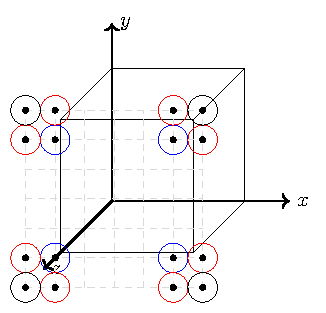
\includegraphics[]{imgs/cqlbm/special cases 3D.pdf}
% \begin{tikzpicture} 
% 		[cube/.style={black},
% 			grid/.style={thin, dashed,color=gray!30},
% 			axis/.style={->,black, thick}]

% 	%draw a grid in the x-y plane

% 	%draw the axes
% 	\draw[axis] (0,0,0) -- (3,0,0) node[anchor=west]{$x$};
% 	\draw[axis] (0,0,0) -- (0,3,0) node[anchor=west]{$y$};
% 	\draw[axis] (0,0,0) -- (0,0,3) node[anchor=west]{$z$};
	
% 	%draw the top and bottom of the cube
% 	\draw[cube] (0,0,0) -- (0,2.25,0) -- (2.25,2.25,0) -- (2.25,0,0) -- cycle;
% 	\draw[cube] (0,0,2.25) -- (0,2.25,2.25) -- (2.25,2.25,2.25) -- (2.25,0,2.25) -- cycle;
	
% 	%draw the edges of the cube
% 	\draw[cube] (0,0,0) -- (0,0,2.25);
% 	\draw[cube] (0,2.25,0) -- (0,2.25,2.25);
% 	\draw[cube] (2.25,0,0) -- (2.25,0,2.25);
% 	\draw[cube] (2.25,2.25,0) -- (2.25,2.25,2.25);

% 	\foreach \x in {-.5,0,...,2.5}
% 		\foreach \y in {-.5,0,...,2.5}
% 		{
% 			\draw[grid] (\x,-.5,2.5 ) -- (\x,2.5,2.5);
% 			\draw[grid] (-.5,\y,2.5) -- (2.5,\y,2.5 );
% 		}
		
% 	\draw[color=green] (2,2,2.5) ellipse (.25cm and .25cm);
%     \node at (2,2,2.5)[circle, fill, color = black, inner sep=1pt]{};
    
%     \draw[color=green] (0,2,2.5) ellipse (.25cm and .25cm);
%     \node at (0,2,2.5)[circle, fill, color = black, inner sep=1pt]{};
    
%     \draw[color=green] (2,0,2.5) ellipse (.25cm and .25cm);
%     \node at (2,0,2.5)[circle, fill, color = black, inner sep=1pt]{};
    
%     \draw[color=green] (0,0,2.5) ellipse (.25cm and .25cm);
%     \node at (0,0,2.5)[circle, fill, color = black, inner sep=1pt]{};
    
%     \draw[color=red] (2,2.5,2.5) ellipse (.25cm and .25cm);
%     \node at (2,2.5,2.5)[circle, fill, color = black, inner sep=1pt]{};
    
%     \draw[color=red] (0,2.5,2.5) ellipse (.25cm and .25cm);
%     \node at (0,2.5,2.5)[circle, fill, color = black, inner sep=1pt]{};
    
%     \draw[color=red] (2,-.5,2.5) ellipse (.25cm and .25cm);
%     \node at (2,-.5,2.5)[circle, fill, color = black, inner sep=1pt]{};
    
%     \draw[color=red] (0,-0.5,2.5) ellipse (.25cm and .25cm);
%     \node at (0,-.5,2.5)[circle, fill, color = black, inner sep=1pt]{};
    
    
%     \draw[color=red] (2.5,2,2.5) ellipse (.25cm and .25cm);
%     \node at (2.5,2,2.5)[circle, fill, color = black, inner sep=1pt]{};
    
%     \draw[color=red] (-.5,2,2.5) ellipse (.25cm and .25cm);
%     \node at (-0.5,2,2.5)[circle, fill, color = black, inner sep=1pt]{};
    
%     \draw[color=red] (2.5,0,2.5) ellipse (.25cm and .25cm);
%     \node at (-.5,0,2.5)[circle, fill, color = black, inner sep=1pt]{};
    
%     \draw[color=red] (-.5,0,2.5) ellipse (.25cm and .25cm);
%     \node at (2.5,0,2.5)[circle, fill, color = black, inner sep=1pt]{};
    
%     \draw[color=black] (2.5,2.5,2.5) ellipse (.25cm and .25cm);
%     \node at (2.5,2.5,2.5)[circle, fill, color = black, inner sep=1pt]{};
    
%     \draw[color=black] (-0.5,2.5,2.5) ellipse (.25cm and .25cm);
%     \node at (-0.5,2.5,2.5)[circle, fill, color = black, inner sep=1pt]{};
    
%     \draw[color=black] (2.5,-0.5,2.5) ellipse (.25cm and .25cm);
%     \node at (2.5,-0.5,2.5)[circle, fill, color = black, inner sep=1pt]{};
    
%     \draw[color=black] (-.5,-0.5,2.5) ellipse (.25cm and .25cm);
%     \node at (-.5,-.5,2.5)[circle, fill, color = black, inner sep=1pt]{};
			
% % 	%draw the top and bottom of the cube
% % 	\draw[cube] (0.5,0.5,0.5) -- (0.5,2.5,.5) -- (2.5,2.5,0.5) -- (2.5,0.5,0.5) -- cycle;
% % 	\draw[cube] (0.5,0.5,2.5) -- (0.5,2.5,2.5) -- (2.5,2.5,2.5) -- (2.5,0.5,2.5) -- cycle;
	
% % 	%draw the edges of the cube
% % 	\draw[cube] (0.5,0.5,0.5) -- (0.5,0.5,2.5);
% % 	\draw[cube] (0.5,2.5,0.5) -- (0.5,2.5,2.5);
% % 	\draw[cube] (2.5,0.5,0.5) -- (2.5,0.5,2.5);
% % 	\draw[cube] (2.5,2.5,0.5) -- (2.5,2.5,2.5);
	
% \end{tikzpicture}
\caption{Illustration of the corner cases specific to a three-dimensional obstacle. The action applied to the different color-coded grid points is described in Section \ref{ssec:spec ref 3d}.}\label{fig:3dpict}
\end{figure}

\begin{figure}[h]
    \centering
    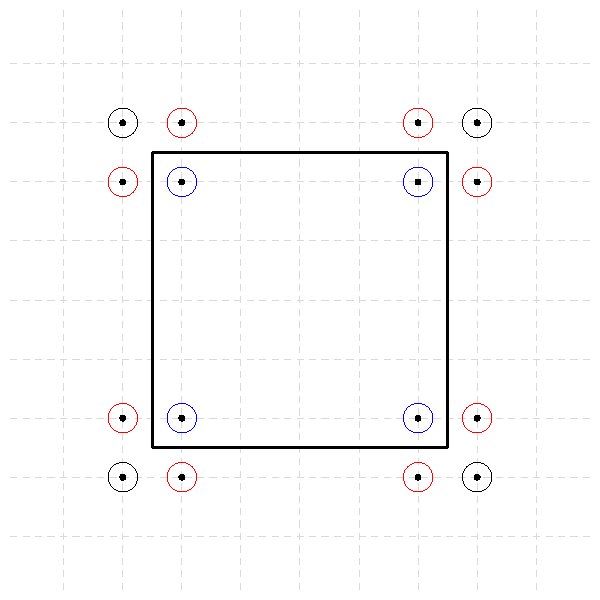
\includegraphics[]{imgs/cqlbm/special cases 3D 2.pdf}
    % \begin{tikzpicture}
    % \draw[help lines, color=gray!30, dashed] (-4.9,-4.9) grid (4.9,4.9);
    % \draw[-,color=black] (-2.5,-2.5) -- (-2.5,2.5);
    % \draw[-,color=black] (-2.5,-2.5) -- (2.5,-2.5);
    % \draw[-,color=black] (2.5,-2.5) -- (2.5,2.5);
    % \draw[-,color=black] (-2.5,2.5) -- (2.5,2.5);
    % \foreach \j in {0,1}
    % {
    %     \foreach \i in {0,1}
    %     {
    %         \node at (-3+\i,-3+\j)[circle, fill, color = black, inner sep=1pt]{};
    %         \node at (2+\i,-3+\j)[circle, fill, color = black, inner sep=1pt]{};
    %     }
    % }
    
    % \foreach \j in {5,6}
    % {
    %     \foreach \i in {0,1}
    %     {
    %         \node at (-3+\i,-3+\j)[circle, fill, color = black, inner sep=1pt]{};
    %         \node at (2+\i,-3+\j)[circle, fill, color = black, inner sep=1pt]{};
    %     }
    % }
    
    % \foreach \j in {0,1}
    % {
    %     \foreach \i in {0,...,4}
    %     {
    %      %   \node at (-1+\i,-3+\j)[circle, fill, color = black, inner sep=1pt]{};
    %      %  \node at (-1+\i,2+\j)[circle, fill, color = black, inner sep=1pt]{};
    %     }
    % }


    % \foreach \i in {0,1}
    % {
    %     \draw[color=black] (-6*\i+3,-6*\i+3) ellipse (.25cm and .25cm);
    %     \draw[color=black] (6*\i-3,-6*\i+3) ellipse (.25cm and .25cm);
        
    %   % \draw[->, dashed, color=green] (2-4*\i,2-4*\i) --  (-5*\i+2.5,-5*\i+2.5);
    %   % \draw[->, dashed, color=green] (-2+4*\i,2-4*\i) -- (5*\i-2.5,-5*\i+2.5);
        
        
        
    %     \draw[color=green] (2,2) ellipse (.25cm and .25cm);
    %     \draw[color=red] (3-1*\i,2+\i) ellipse (.25cm and .25cm) ;
    %     %\draw[->, color=blue] (2,2) --  (2+1*\i,3-\i);
        
    %     \draw[color=green] (-2,2) ellipse (.25cm and .25cm);
    %     \draw[color=red] (-2-1*\i,3-\i) ellipse (.25cm and .25cm);
        
    %     \draw[color=green] (-2,-2) ellipse (.25cm and .25cm);
    %     \draw[color=red] (-2-1*\i,-3+\i) ellipse (.25cm and .25cm);
        
    %     \draw[color=green] (2,-2) ellipse (.25cm and .25cm);
    %     \draw[color=red] (2+\i,-3+\i) ellipse (.25cm and .25cm);
        
    %     %\draw[->, color=red] (2,2) --  (3-2*\i,1+2*\i);
    %     % \draw[->, dashed, color=red] (2,2) --  (2.5 -\i,1.5+\i);
    %     % \draw[->,  color=red] (3 -2*\i,1+2*\i) --  (2.5 -\i,1.5+\i);
        
        
    %     % \draw[->, dashed, color=red] (-2,2) --  (-2.5+\i,1.5+\i);
    %     % \draw[->, color=red] (-3+2*\i,1+2*\i) -- (-2.5+\i,1.5+\i);
        
    %     % \draw[->, dashed, color=red] (-2,-2) --  (-2.5+\i,-1.5-\i);
    %     % \draw[->, color=red] (-3+2*\i,-1-2*\i) --  (-2.5+\i,-1.5-\i);
        
    %     % \draw[->, dashed, color=red] (2,-2) --  (2.5-\i,-1.5-\i);
    %     % \draw[->, color=red] (3-2*\i,-1-2*\i) --  (2.5-\i,-1.5-\i);
    % }
    % \end{tikzpicture}
    \caption{View from the positive $z$-axis onto the $xy$-wall of the obstacle. Note that the $xy$-wall lies half a grid point in the z-direction below the grid with the encircled points. 
 }\label{fig:3dpictin2d}
\end{figure}


% \begin{tikzpicture}[scale=3,tdplot_rotated_coords,
%                     cube/.style={very thick,black},
%                     grid/.style={very thin,gray},
%                     axis/.style={->,blue,ultra thick},
%                     rotated axis/.style={->,purple,ultra thick}]

%     %draw a grid in the x-y plane
%     \foreach \x in {-0.5,0,...,2.5}
%         \foreach \y in {-0.5,0,...,2.5}
%         {
%             \draw[grid] (\x,-0.5) -- (\x,2.5);
%             \draw[grid] (-0.5,\y) -- (2.5,\y);
%         }

%     %draw the main coordinate frame axes
%     \draw[axis,tdplot_main_coords] (0,0,0) -- (3.5,0,0) node[anchor=west]{$x$};
%     \draw[axis,tdplot_main_coords] (0,0,0) -- (0,3.5,0) node[anchor=north west]{$y$};
%     \draw[axis,tdplot_main_coords] (0,0,0) -- (0,0,3.5) node[anchor=west]{$z$};


%     %draw the rotated coordinate frame axes
%     % \draw[rotated axis] (0,0,0) -- (3,0,0) node[anchor=west]{$x'$};
%     % \draw[rotated axis] (0,0,0) -- (0,3,0) node[anchor=south west]{$y'$};
%     % \draw[rotated axis] (0,0,0) -- (0,0,3) node[anchor=west]{$z'$};

%     %draw the top and bottom of the cube
%     \draw[cube] (0,0,0) -- (0,2,0) -- (2,2,0) -- (2,0,0) -- cycle;

%     %draw the top and bottom of the cube
%     \draw[cube] (0,0,0) -- (0,2,0) -- (0,2,2) -- (0,0,2) -- cycle;

%     %draw the top and bottom of the cube
%     \draw[cube] (0,0,0) -- (2,0,0) -- (2,0,2) -- (0,0,2) -- cycle;

% \foreach \x in {0,1,2}
%   \foreach \y in {0,1,2}
%       \foreach \z in {0,1,2}{
%           %#####################################################
%           \ifthenelse{  \lengthtest{\x pt < 2pt}  }
%           {
%              % True
%                 \draw [black]   (\x,\y,\z) -- (\x+1,\y,\z);
%           }
%           {% False
%           }
%           %#####################################################
%           \ifthenelse{  \lengthtest{\y pt < 2pt}  }
%           {
%              % True
%                 \draw [black]   (\x,\y,\z) -- (\x,\y+1,\z);
%           }
%           {% False
%           }
%           %#####################################################
%           \ifthenelse{  \lengthtest{\z pt < 2pt}  }
%           {
%              % True
%                 \draw [black]   (\x,\y,\z) -- (\x,\y,\z+1);
%           }
%           {% False
%           }
%           %\shade[rotated axis,ball color = purple!80] (\x,\y,\z) circle (0.06cm);          
% }

% \end{tikzpicture}




\subsubsection{Efficient object encoding}
% In order to ensure polynomial complexity of our algorithm, we need to be able to determine whether or not a grid point is part of a given wall (or right outside the wall) in polynomial time. 
% This can be done trivially if we simply assume that the size of the walls grow, for instance, with a constant parameter of the amount of qubits used to encode the grid in a given dimension. This assumption, however, is highly restrictive. As this would imply that the amount of grid points grows exponentially with the amount of qubits (as it always does), but the wall size grows linearly. When adding more qubits to the system we then simply end up with a very small object in a very large space. And when assuming that the size of a wall grows linearly in the amount of grid points as is done in \cite{Todorova2020}, this assumption implies that the size of the wall grows exponentially in the amount of qubits required to encode the grid. Since we want to avoid exponential growth of the circuit in the number of qubits as well as an assumption leading to an unnatural restriction in object size, we propose a method that shows we can determine whether or not a grid is part of a wall in polynomial time for any given wall size. \\


In this section we propose a novel approach based on quantum comparison operations for encoding objects in a way that we can efficiently identify whether or not a grid point is part of a certain object wall. Our approach requires $2(d-1)$ extra ancillae and will be explained at the hand of a two-dimensional example.


% \xout{In this section we provide a novel quantum approach for encoding objects that can efficiently identify whether or not a grid point is part of a certain wall of an object.}

% \xout{We do this by making use of quantum comparison operations in combination with $2(d-1)$ extra ancillae. 
% We explain how to use this method via an example in the two-dimensional case.} \\

% \xout{In the two-dimensional case we use the quantum comparison method as follows. }
Assume that we want to encode a $y$-wall (note that everything works the same to encode an $x$-wall), for example the left-most $y$-wall of Figure \ref{fig:example_right}. Let the grid points just inside the object next to the $y$-wall, i.e., the left-most blue encircled grid points inside the object of Figure \ref{fig:example_right}, range from $[ a,b ]$ in the $y$-axis. We first need to determine whether or not we are in one of the left-most blue encircled grid points inside the object with the aid of two quantum comparison operations. The first quantum comparison operation checks whether $y \geq l$ holds. If so we flip the first extra ancilla from its start state $a_{a,1}= 0$ to $a_{a,1}= 1$. Then we check if $y \leq u$ holds, and if so we flip the second extra ancilla to $a_{b,1}= 1$. Now, controlled on these both ancillae and the state of the qubits encoding the position in the $x$ dimension of these left-most blue encircled qubits, we flip the ancilla $a_{o,x}$ indicating that we are in a wall which reflects the velocity in the $x$-direction.
Now we simply reset the $a_{a,1}$ and $a_{b,1}$ ancillae so that they can be reused for other walls, by performing the same quantum comparison operations as described before\footnote{Note that in the example of Figure \ref{fig:example_right} it would be most efficient to first flip the ancilla $a_{o,x}$ as well, controlled on the $a_{a,1}$ and $a_{b,1}$ qubits in combination with the qubits encoding the position in the $x$ dimension being in the position of the right-most blue encircled grid points inside the object. But for now we were only considering the left-most $y$-wall.}.
In the two-dimensional case we perform this operation for all walls in order to set the $a_{o,x}$ and $a_{o,y}$ qubits as required. After completion of this step we continue in the same fashion as described in Section \ref{ssec:Correct Reflection}.

What remains is to reset the $a_{o,x}$ and $a_{o,y}$ qubits after the reflection and streaming steps have been performed which we accomplish, again, with the aid of the quantum comparison operation. To continue with our example of the left-most $y$-wall of Figure \ref{fig:example_right}, we again perform two comparison operations to check whether we are in the left-most blue encircled grid points right outside the wall, which amounts to checking $y \in [l+1,u-1]$. This can be achieved with the same logic as before namely by checking $y \geq l+1$ and $y \leq u-1$. All the other steps and the resetting are performed in the same manner as explained before. The extension to the three-dimensional case is straightforward.






\subsubsection{Quantum Comparison Operation}\label{ssec: quantum comparison}
In our implementation we use the quantum comparison operation from \cite{Gidney2017}, which compares the integer value $i$ of the $n$-qubit quantum state $\ket{i}$ with a pre-determined constant $k$ saving the result of the comparison in a separate qubit. 

% The operation consists of one (periodic) subtraction operation defined on the total $n$+1 qubits followed by a (periodic) addition defined on the $n$ qubits encoding the original quantum state. Multiple realizations of quantum addition and subtraction operations are described in the literature \cite{Häner2017,Takahashi2009,Cuccaro2004,Draper1998}, all having their own complexities and required ancillae associated to them.

The quantum comparison algorithm works as follows. Say we wish to determine whether the integer value $i$ encoded in basis state $\ket{i}$ is smaller than $k$\footnote{Note that $k \leq 2^n-1$ always holds, since otherwise we trivially know that $k$ is larger than any value that $n$ qubits can encode.}. Then, we first subtract the integer $k$ from the value encoded by the $n+1$ qubits encoding the state $\ket{0}\otimes\ket{i}$, where the prepended $\ket{0}$ qubit will hold the result of the computation. Now there are two cases, $i\geq k$ and $i<k$. \\

Assume that we are in the case $i \geq k$. Then subtracting $k$ from $i$ encoded in  $\ket{0}\otimes\ket{i}$ gives $\ket{0}\otimes \ket{i-k}$, which leaves the prepended $\ket{0}$ qubit unchanged. 
Now we simply perform an addition of the value $k$ to the $n$-qubits that are used to encode $i$ and now encode $\ket{i-k}$. This gives $\ket{0}\otimes\ket{i-k+k} = \ket{i}$. And so in total we end up with a quantum register in the state $\ket{0}\otimes\ket{i}$. Where the $\ket{0}$ state is the result of the computation which means that $i \geq k$ in fact holds, and the last $n$ qubits are again in the original state $\ket{i}$. \\

Now let us assume that we are in the second case $i<k$. Again, we start by periodically subtracting the integer $k$ from $i$ encoded in the state $\ket{0}\otimes\ket{i}$, only now since $k>i$ we end up flipping the state of the prepended $\ket{0}$ qubit. This is because periodically subtracting $k$ from $i$ in a state encoded by $n+1$ qubits results in the state $\ket{2^{n+1} -1 - k +i}$. Since $k \leq 2^n-1$ and $i \geq 0$ we must have that $2^{n+1} -1 - k +i \geq 2^n$ and so the state of the most significant qubit must be equal to $\ket{1}$. This means that the total qubit register is now in the state $\ket{1} \otimes \ket{2^{n+1} -1 - k +i - 2^n} =\ket{1} \otimes \ket{2^{n} -1 - k +i }  $. 

Then, as before, we simply add the integer $k$ again to the last $n$ qubits of the register leaving us with $\ket{1} \otimes \ket{2^{n} -1 +i } = \ket{1} \otimes \ket{ i } $ due to periodicity. Notice how the most significant qubit is left in the state $\ket{1}$ indicating that in fact $k > i$, whilst again the qubits encoding $\ket{i}$ have not changed.  \\

Multiple realizations of quantum addition and subtraction operations are described in the literature \cite{Häner2017,Takahashi2009,Cuccaro2004,Draper1998} and can be used for the comparison operation, all having their own complexities and required ancillae associated to them. \\

A quantum primitive for checking whether $i\geq k$ holds can be easily designed from the above ($i<k$) by simply negating the qubit that holds the result after performing $i<k$. 

Implementing a quantum primitive that determines $i\leq k$ is a bit more involved as we need to consider two different cases. First, if $k = 2^n -1$ simply flip the ancilla holding the result, as $i \leq k$ trivially holds, otherwise we can implement $i< k+1$ to get the desired result. Notice that here we can easily implement this two case method for $i \leq k$ since $k$ is an integer determined before the running of the algorithm. 


\subsection{Quantum bounce back boundary conditions}\label{sec:qbb}
One of the most commonly used boundary conditions in practical LBM is the bounce back boundary condition which amounts to fully reflecting the direction of particles that get into contact with obstacles and resetting them to their original position inside the flow domain \cite{Schiller2008, Kruger2017}. This is different from the specular reflection boundary conditions that we adopted in our earlier work \cite{Schalkers2022}, which reverses only the normal component of the velocity vector. Figure \ref{fig:bounce_back_vs_specular_reflection} illustrates the difference between the two types of boundary conditions, where specular reflection takes places between grid positions 2 and 3 on $x$ axis, while bounceback occurs between positions 4 and 5. 

The algorithm for implementing bounce back boundary conditions in a classical LBM can be summarized as follows. First, the particles that virtually travelled into the obstacle have their velocity direction reversed in all dimensions and subsequently these particles are placed outside of the obstacle. The particles are placed in the correct position outside of the obstacle by moving one point in the dimension(s) that they previously moved in. 

\begin{figure}[h]
    \centering
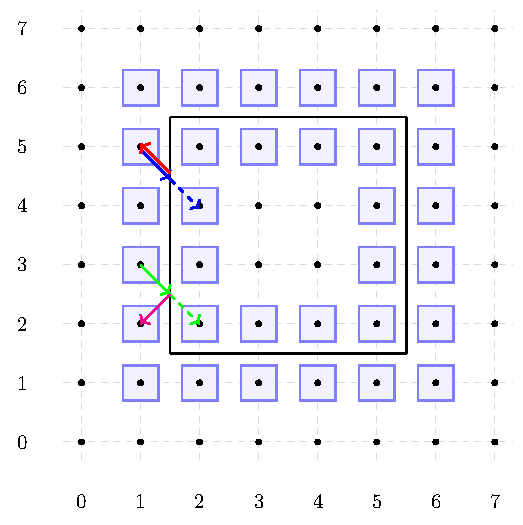
\includegraphics[]{imgs/cqlbm/bounceback_plaatje.pdf}
    \caption{Illustration of bounce back boundary conditions (top, in red and blue arrows) versus specular reflection boundary conditions (bottom, in green and magenta).}
    \label{fig:bounce_back_vs_specular_reflection}
\end{figure}

For implementing the bounce back boundary condition as a quantum primitive we require only one ancilla qubit $a_{o}$ to indicate whether a particle has virtually moved into an object. The ancilla $a_{o}$ is initialized in the $\ket{0}$ state and flipped to $\ket{1}$ when a particle has virtually travelled into one of the points inside the obstacle. We check whether a particle has virtually travelled into the object using the efficient object encoding method as described in Section \ref{sec:complete quantum specular reflection step}. 

As a next step we flip the state of the $v_\text{dir}^j$ qubits for all dimensions $j$ controlled on the state of the $a_o$ ancilla. By doing this we make sure that the velocity direction is reversed in all dimensions after contact with an obstacle as is required for bounce back boundary conditions. And subsequently the particles are moved by one position controlled on the $a_v^j$ , $v_\text{dir}^j$ and $a_o$ qubits to ensure that the particles move one step in the correct direction in the dimension(s) that they moved in when they moved into the obstacle and of course to ensure that this only happens after the particles moved into the obstacle. 

Finally the $a_o$ qubits need to be reset to $\ket{0}$ before we can start the next time step. As in Section \ref{sec:complete quantum specular reflection step} the blue and green encircled points outside of the object constitute the trivial case in Figure \ref{fig:example_right}. We reset the $a_o$ qubits controlled on if we are in one of the blue (green) encircled points, the direction of the $x$ ($y$) velocity and the ancilla qubit indicating whether we moved in the dimension in this time step $a_v^1$ ($a_v^2$). Specifically we reset the ancilla qubit $a_o$ if we are in a blue (green) encircled grid point outside the object and $a_v^1 = 1$ ($a_v^2 = 1$) and $v_\text{dir}^1$ ($v_\text{dir}^2$) points away from the object. Using this logic the $a_o$ qubits are reset to $\ket{0}$ for each wall separately.

Resetting the $a_o$ qubit is a bit more difficult around the edges as indicated with black and orange encircled points in Figure \ref{fig:example_right}. 

For the black encircled points outside the corner we need to reset the ancilla qubit $a_o$ if and only if both $v_\text{dir}^1$ and $v_\text{dir}^2$ point in the direction away from the object and $a_v^1 = a_v^2 =1$ holds.

As for the orange encircled `side-edge' grid point we first reset the $a_o$ ancilla in the same way as for the blue (green) encircled points described above. Now we only need to note that for the case described by the red arrow in Figure \ref{fig:example_right} we have wrongly flipped the $a_o$ ancilla qubit and so we need to verify whether we are in the `red arrow' case by checking if $v_\text{dir}^1$ and $v_\text{dir}^2$ pointed in the direction of the arrow and if $a_v^1 = a_v^2 =1$ holds. If the particle is in a state where  $a_v^1 = a_v^2 =1$ and $v_\text{dir}^1$ and $v_\text{dir}^2$ are such that the particle is in an red arrow case the $a_o$ ancilla get flipped again, back to the original state of $\ket{0}$. 

\begin{figure}[h]
    \centering
    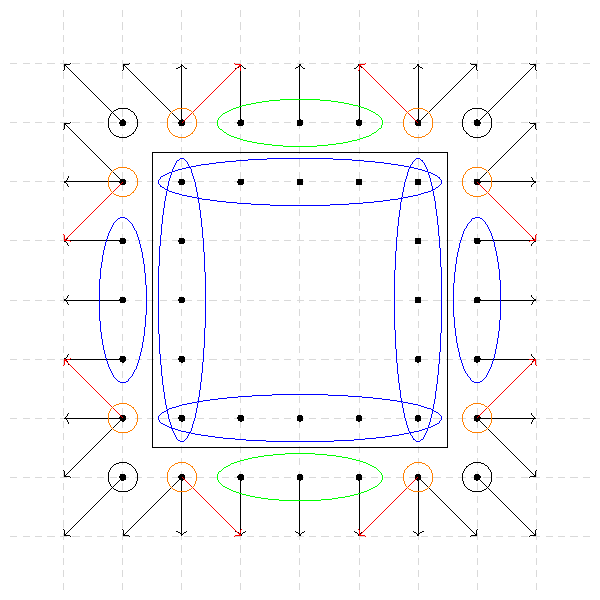
\includegraphics[]{imgs/cqlbm/corner_cases_bb.pdf}
    \caption{Illustration of all possible corner cases to be taken into account when particles collide with an obstacle (black box) and the physically correct behavior for a fail-safe implementation of boundary conditions.}
    \label{fig:example_right}
\end{figure}


\section{Quantum momentum exchange method}\label{sec:QMEM}
In this section we explain how the momentum exchange method can be expressed as an observable for the encoding described in Section \ref{sec:quantum register set-up}. In order to do this we will first change the density encoding of the quantum state into a rooted density encoding. Using this rooted density encoding we can subsequently define the observable that calculates the force using Equation \eqref{eq:F2} and finally we describe how this method can be implemented as an executable quantum circuit.

\paragraph*{Rooted density encoding}\label{subseq:rooted}
Since the momentum exchange method is linear in nature, whereas quantum observables are quadratic, it is advisable to change from encoding the density function $ f_i \left  (\mathbf{x},t \right ) $ in the quantum state $\ket{\psi}$ to an encoding of the square root of the density function $\sqrt{ f_i \left ( \mathbf{x}, t \right ) }$. Such a shift to a rooted density encoding can be done without altering any subsequent circuits in the methods \cite{Schalkers2022, Todorova2020}. 


\subsection{Momentum exchange method as an observable}\label{subseq:obs}
We now derive the observable that calculates the force exerted on the object using the momentum exchange method. As force is described using a vector, we need to calculate the values of the vector for all $d$ dimensions. Here we show how to calculate this vector using $2d$ different observables, where each observable calculates the value of the force vector in one spatial dimension, $d\in\{1,2,3\}$, and one velocity direction. This is done to make the resulting observable easier to portray and explain, since all the observables can be expressed as diagonal matrices they do commute and so they can all be measured in the same runs. 

Considering the encoding described above, Equation \eqref{eq:F2} can be evaluated from the quantum state $\ket{\psi}$ encoding $\sqrt{ f_i \left (\mathbf{x},t \right )}$, by the diagonal observable $O_{\text{OME}}$ to be specified below. The diagonal of the matrix expressing the observable $O_\text{OME}$ is built up using $B_{\text{OME}}$ matrices, which are placed at grid points in the fluid domain directly adjacent to the obstacle. All the other indices of the matrix matrix expressing $O_{\text{OME}}$ will remain zero. An example of this is the matrix
\begin{equation}\label{eq:Obs_1}
        O_{\text{OME}} = \begin{bmatrix}
            \dots & \dots & \dots & \dots  \\
            \dots &  B_{\text{OME}} & \dots & \dots \\
            \dots & \dots & \dots & \dots \\
            \dots & \dots & \dots & \dots \\
        \end{bmatrix},
\end{equation}
where the dots represent $4 \times 4$ matrices with only 0 indices and $B_{\text{OME}}$ is a $4 \times 4$ matrix that can be written as 
\begin{equation}\label{eq:bmatrix}
    B_{\text{OME}} = \begin{bmatrix}
        0 & 0 & 0 & 0\\
        0 & 0 & 0 & 0 \\
        0 & 0 & 2 & 0 \\
        0 & 0 & 0 & 0 
    \end{bmatrix}.
\end{equation}
The example given in Equation \eqref{eq:Obs_1} represents a 1-dimensional case with 4 grid points and three possible speeds (one in the positive and one in the negative $x$-direction as well as the zero speed) and the wall adjacent to the second grid point as represented in Figure \ref{fig:D1Q3ex_obs}. Since $B_{\text{OME}} = B_{\text{OME}}^{\dagger}$, both $B_{\text{OME}}$ and $O_{\text{OME}}$ are Hermitian and therefore $O_{\text{OME}}$ constitutes a quantum observable. It can easily be seen that any other distribution of $B_{\text{OME}}$ along the diagonal will also lead to a quantum observable. 

\begin{figure}[h]
    \centering
    
\includegraphics[]{imgs/cqlbm/four_gp_1_box.pdf}
\caption{Example of the D1Q3 case with four grid points and one obstacle located on the third grid point.}
\end{figure}\label{fig:D1Q3ex_obs}

For the D1Q3 case with four grid points described above we have the following quantum state encoding \begin{equation} \ket{\psi} = \frac{1}{\sqrt{\sum_{x,i} f_i \left (\mathbf{x},t \right )}} \sum_{x,i} \sqrt{ f_i \left (\mathbf{x} ,t \right )}\ket{g^1_2g^1_1v^1v^1_\text{dir}},
\end{equation} where $g^1_2g^1_1$ represent the binary value of the location of the $x$-axis, $\ket{v^1v^1_\text{dir}} = 01$ indicates streaming in the positive $x$-direction, $\ket{v^1v^1_\text{dir}}=11$ indicates streaming in the negative $x$-direction and $\ket{v^1v^1_\text{dir}}=01$ as well as $\ket{v^1v^1_\text{dir}}=00$ indicates that the particle is not streaming in the $x$-direction. Here and in the remainder of this Section we do not take into account the ancilla qubits as they play no role in the final density function and as such will not be part of the measurement process.

With the above convention, the quantum state can be written as the coefficient vector relative to the computational basis as follows: 
\begin{equation}\label{eq:psi}
    \ket{\psi} = \sum_{x,v} \alpha_{x,v} \ket{g^1_2g^1_1v^1v^1_\text{dir}} = \frac{1}{\sqrt{\sum_{x,i} f_i \left (\mathbf{x},t \right )}} \begin{bmatrix}
        0 \\
        \sqrt{f_0(0,t)} \\
        \sqrt{f_1(0,t)} \\
        \sqrt{f_2(0,t)} \\
        0 \\
        \sqrt{f_0(1,t)} \\
        \sqrt{f_1(1,t)} \\
        \sqrt{f_2(1,t)} \\
        0 \\
        \sqrt{f_0(2,t)} \\
        \sqrt{f_1(2,t)} \\
        \sqrt{f_2(2,t)} \\
        0 \\
        \sqrt{f_0(3,t)}  \\ 
        \sqrt{f_1(3,t)} \\
        \sqrt{f_2(3,t)}         
        % \sqrt{f(0,v_0)} \\
        % \sqrt{f(0,v_1)} \\
        % \sqrt{f(1,v_0)} \\
        % \sqrt{f(1,v_1)} \\
        % \sqrt{f(2,v_0)} \\
        % \sqrt{f(2,v_1)} \\
        % \sqrt{f(3,v_0)} \\
        % \sqrt{f(3,v_1)}      
    \end{bmatrix}.
\end{equation}
Using expression \eqref{eq:psi} and some basic linear algebra it follows that
\begin{equation}\label{eq:obs_value}
    \braket{\psi|O_{\text{OME}}|\psi} = \frac{2f_1 \left ( 1, t \right )}{\sum_{x,i}f_i \left (\mathbf{x},t \right )} .
\end{equation}
Since the value of $\sum_{x,i}f_i \left (\mathbf{x},t \right )$ is known when starting the algorithm we can simply multiply Equation \eqref{eq:obs_value} by $\sum_{x,i}f_i \left (\mathbf{x},t \right )$ to find the value of the force we wish to calculate as described in Equation \eqref{eq:F2}, which can subsequently be used to calculate the drag and lift coefficient \cite{Ladd1994}. 

\paragraph*{Extension to more dimensions}
This method can easily be extended to more dimensions by noticing that the $B_\text{OME}$ matrix is of size $2^{n_v} \times 2^{n_v}$ and should consist of only one non-zero element. This non-zero element will always be placed on the diagonal at the position of the basis state $\ket{v^i}$. 

\paragraph*{Complexity Analysis}\label{sec:CA}
The number of measurements required to determine the force with an $\epsilon$ precision using our proposed approaches depends on multiple factors. 
As long as the total number of grid points located inside and adjacent to the boundary of the obstacle is polynomial in the total number of grid points, the number of diagonal elements that are non-zero in the observable is polynomial in the size of the grid. This means that the number of non-zero elements in the observable is not exponentially small in the total size of the system. Therefore, in this case, we wish to measure a subspace that is only polynomially small in the total size of the system which is feasible without exponential overhead. 

\subsection{Practical implementation of the momentum exchange method on a quantum computer}\label{sec:prac_impl}
Realizing an observable on a real-world quantum computer amounts to implementing a quantum circuit that translates the observable to measurements in the computational Z-basis.
We will now present the quantum circuit that translates the observable described in Subsection \ref{subseq:obs} for determining the force in one dimension in one direction to measuring one qubit in the Z-basis, making the process clear and easily implementable on a quantum device. 

We will first describe how this operation can be applied by using an already implemented circuit for the bounce back boundary condition and we will subsequently show that this operation indeed transforms the described observable to one that consists of a Z measurement on one qubit. 

\subsubsection{Implementation using ancilla qubits for bounce back boundary conditions}
We have implemented a method to measure the expectation value of the described observable by measuring only one qubit. This is done using the implementation of the bounce back boundary conditions. In this implementation a qubit $a_{o}$ gets flipped to indicate that a particle is inside an object. To determine the expectation value of the observable we will use these ancilla qubits differently. We will from now on call this $a_{o}$ ancilla qubit that was used for the bounce back boundary conditions $a_{o,+}$ and we define a second ancilla qubit $a_{o,-}$. These ancilla qubits will be flipped if a force was exerted on the object in a positive or negative direction, respectively. In order to do this we apply a multi-controlled NOT operation controlled on the  qubits to determine whether we are in the object and the qubit indicating the direction of the particles in the dimension to the $a_{o,+}$ ($a_{o,-}$) qubits.  

By doing this we are extracting the relative density of particles that come into contact with an obstacle in the positive and negative direction for the considered dimension. Subsequently we measure the qubits $a_{o,+}$ and $a_{o,-}$ and subtract the expectation value of $a_{o,-}=1$ from $a_{o,+} = 1$. The resulting value expresses the relative pressure in the positive / negative direction. 

\subsubsection{Proof of method}
In this section we show that using the method described above, we indeed calculate the force exerted on an object in one dimension as expressed in Equation \eqref{eq:F2}.

We flip the $a_{o,+}$ ancilla qubit in the case that particles have impinged on the object and the particles have a positive velocity in the $x$-direction. %@Merel je hebt er hier x van gemaakt omdat het duidelijker lijkt dan steeds naar de desbetreffende dimensie te refereren. Pas dit later aan.
Therefore, after re-arranging some qubits, we can write 
\begin{equation}
\begin{split}
    & \bigl( \sqrt{f_{v_0} \left ( x_0,t \right )} \ket{ \left ( g_{n_g} \dots g_{1} \right )_0 \left (  v_{n_v} \dots v_1 \right )_0 } + \dots +   \\ & \sqrt{f_{v_1} \left ( x_1, t\right )} \ket{ \left (  g_{n_g} \dots g_{1} \right )_1 \left (  v_{n_v} \dots v_1 \right )_1} \bigr) \ket{0}_{a_{o,+}} +  \\ & \bigl( \sqrt{f_{v_2} \left ( x_2, t \right )}\ket{\left ( g_{n_g} \dots g_{1} \right )_2 \left ( v_{n_v} \dots v_1 \right)_2} + \dots +  \\  & \sqrt{f_{v_3} \left ( x_3 ,t\right )} \ket{ \left ( g_{n_g} \dots g_{1} \right )_3 \left ( v_{n_v} \dots v_1 \right )_3}  \bigr) \ket{1}_{a_{o,+}},
    \end{split}
\end{equation}
where for $v_i$ and $x_i$  the subscript is simply used to indicate that a specific value for the location and velocity is considered and similarly for the qubits $\left ( g_{n_g} \dots g_{1} \right )_i$ $\left (  v_{n_v} \dots v_1 \right )_i$ the subscript is used to indicate the velocity and grid point qubits are in a specific state. 
Here the states $ \ket{ \left ( g_{n_g} \dots g_{1} \right )_0 \left (  v_{n_v} \dots v_1 \right )_0 } + \dots +  \ket{\left (  g_{n_g} \dots g_{1} \right )_1 \left (  v_{n_v} \dots v_1 \right )_1}$ describe exactly the particles that do not impinge on the object in the positive $x$-direction in the current time step, as the $a_{o,+}$ qubit is in the $\ket{0}$ state. Similarly the states $\ket{\left ( g_{n_g} \dots g_{1} \right )_2 \left ( v_{n_v} \dots v_1 \right)_2} + \dots + \ket{\left ( g_{n_g} \dots g_{1} \right )_3 \left ( v_{n_v} \dots v_1 \right )_3}$ represent the relative densities of the particles that have impinged the object in the positive $x$-direction.
From this we can conclude that the total probability of finding $\ket{a_{o,+}} = \ket{1}$ upon measurement is equal to \begin{equation}
    f_{v_2} \left ( x_2, ,t\right ) + \dots + f_{v_3} \left ( x_3,t \right ),
\end{equation}
which is precisely equal to the relative density of particles hitting the object with a positive velocity and which is precisely what we wish to measure. 
